\documentclass[1p]{elsarticle_modified}
%\bibliographystyle{elsarticle-num}

%\usepackage[colorlinks]{hyperref}
%\usepackage{abbrmath_seonhwa} %\Abb, \Ascr, \Acal ,\Abf, \Afrak
\usepackage{amsfonts}
\usepackage{amssymb}
\usepackage{amsmath}
\usepackage{amsthm}
\usepackage{scalefnt}
\usepackage{amsbsy}
\usepackage{kotex}
\usepackage{caption}
\usepackage{subfig}
\usepackage{color}
\usepackage{graphicx}
\usepackage{xcolor} %% white, black, red, green, blue, cyan, magenta, yellow
\usepackage{float}
\usepackage{setspace}
\usepackage{hyperref}

\usepackage{tikz}
\usetikzlibrary{arrows}

\usepackage{multirow}
\usepackage{array} % fixed length table
\usepackage{hhline}

%%%%%%%%%%%%%%%%%%%%%
\makeatletter
\renewcommand*\env@matrix[1][\arraystretch]{%
	\edef\arraystretch{#1}%
	\hskip -\arraycolsep
	\let\@ifnextchar\new@ifnextchar
	\array{*\c@MaxMatrixCols c}}
\makeatother %https://tex.stackexchange.com/questions/14071/how-can-i-increase-the-line-spacing-in-a-matrix
%%%%%%%%%%%%%%%

\usepackage[normalem]{ulem}

\newcommand{\msout}[1]{\ifmmode\text{\sout{\ensuremath{#1}}}\else\sout{#1}\fi}
%SOURCE: \msout is \stkout macro in https://tex.stackexchange.com/questions/20609/strikeout-in-math-mode

\newcommand{\cancel}[1]{
	\ifmmode
	{\color{red}\msout{#1}}
	\else
	{\color{red}\sout{#1}}
	\fi
}

\newcommand{\add}[1]{
	{\color{blue}\uwave{#1}}
}

\newcommand{\replace}[2]{
	\ifmmode
	{\color{red}\msout{#1}}{\color{blue}\uwave{#2}}
	\else
	{\color{red}\sout{#1}}{\color{blue}\uwave{#2}}
	\fi
}

\newcommand{\Sol}{\mathcal{S}} %segment
\newcommand{\D}{D} %diagram
\newcommand{\A}{\mathcal{A}} %arc


%%%%%%%%%%%%%%%%%%%%%%%%%%%%%5 test

\def\sl{\operatorname{\textup{SL}}(2,\Cbb)}
\def\psl{\operatorname{\textup{PSL}}(2,\Cbb)}
\def\quan{\mkern 1mu \triangleright \mkern 1mu}

\theoremstyle{definition}
\newtheorem{thm}{Theorem}[section]
\newtheorem{prop}[thm]{Proposition}
\newtheorem{lem}[thm]{Lemma}
\newtheorem{ques}[thm]{Question}
\newtheorem{cor}[thm]{Corollary}
\newtheorem{defn}[thm]{Definition}
\newtheorem{exam}[thm]{Example}
\newtheorem{rmk}[thm]{Remark}
\newtheorem{alg}[thm]{Algorithm}

\newcommand{\I}{\sqrt{-1}}
\begin{document}

%\begin{frontmatter}
%
%\title{Boundary parabolic representations of knots up to 8 crossings}
%
%%% Group authors per affiliation:
%\author{Yunhi Cho} 
%\address{Department of Mathematics, University of Seoul, Seoul, Korea}
%\ead{yhcho@uos.ac.kr}
%
%
%\author{Seonhwa Kim} %\fnref{s_kim}}
%\address{Center for Geometry and Physics, Institute for Basic Science, Pohang, 37673, Korea}
%\ead{ryeona17@ibs.re.kr}
%
%\author{Hyuk Kim}
%\address{Department of Mathematical Sciences, Seoul National University, Seoul 08826, Korea}
%\ead{hyukkim@snu.ac.kr}
%
%\author{Seokbeom Yoon}
%\address{Department of Mathematical Sciences, Seoul National University, Seoul, 08826,  Korea}
%\ead{sbyoon15@snu.ac.kr}
%
%\begin{abstract}
%We find all boundary parabolic representation of knots up to 8 crossings.
%
%\end{abstract}
%\begin{keyword}
%    \MSC[2010] 57M25 
%\end{keyword}
%
%\end{frontmatter}

%\linenumbers
%\tableofcontents
%
\newcommand\colored[1]{\textcolor{white}{\rule[-0.35ex]{0.8em}{1.4ex}}\kern-0.8em\color{red} #1}%
%\newcommand\colored[1]{\textcolor{white}{ #1}\kern-2.17ex	\textcolor{white}{ #1}\kern-1.81ex	\textcolor{white}{ #1}\kern-2.15ex\color{red}#1	}

{\Large $\underline{12a_{1056}~(K12a_{1056})}$}

\setlength{\tabcolsep}{10pt}
\renewcommand{\arraystretch}{1.6}
\vspace{1cm}\begin{tabular}{m{100pt}>{\centering\arraybackslash}m{274pt}}
\multirow{5}{120pt}{
	\centering
	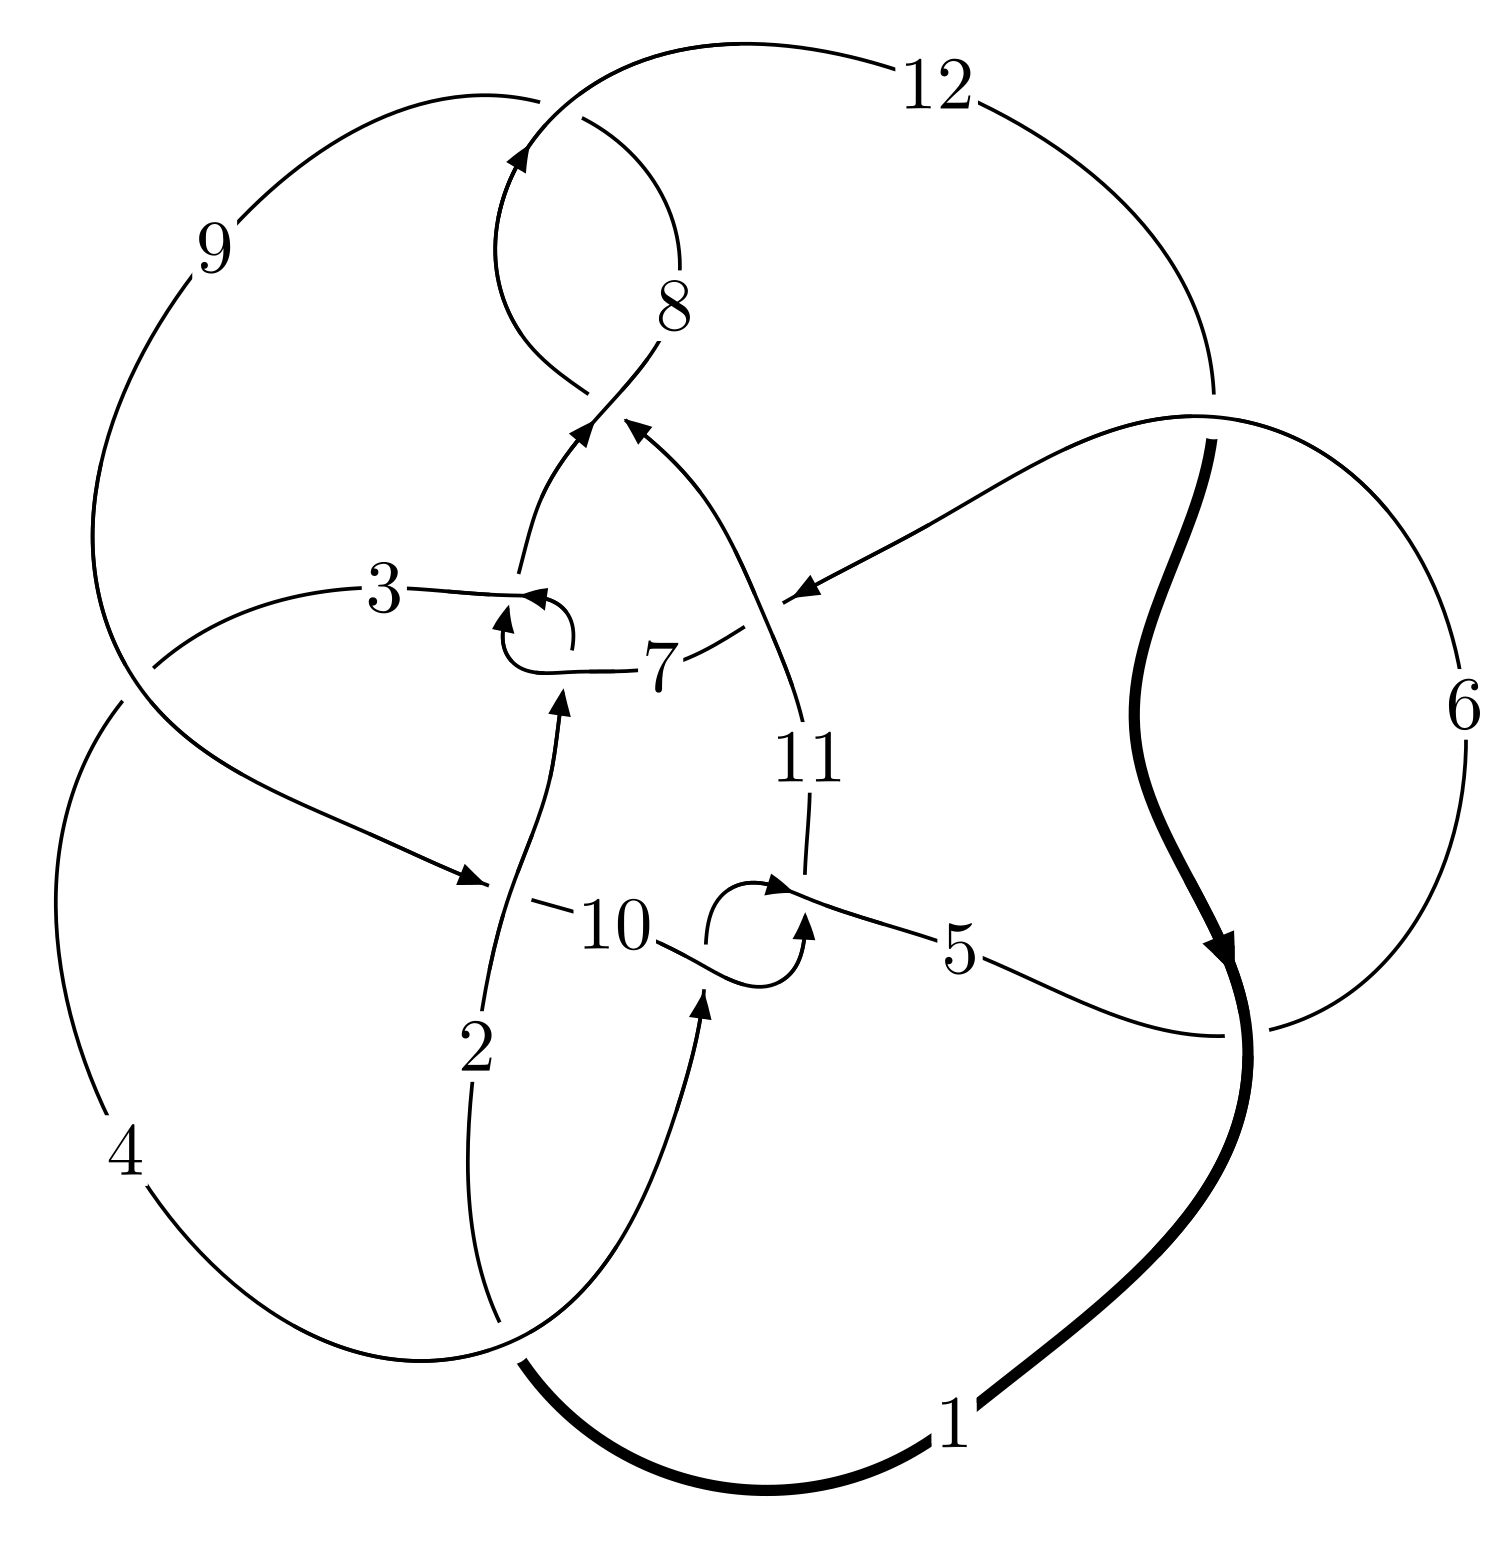
\includegraphics[width=112pt]{../../../GIT/diagram.site/Diagrams/png/1857_12a_1056.png}\\
\ \ \ A knot diagram\footnotemark}&
\allowdisplaybreaks
\textbf{Linearized knot diagam} \\
\cline{2-2}
 &
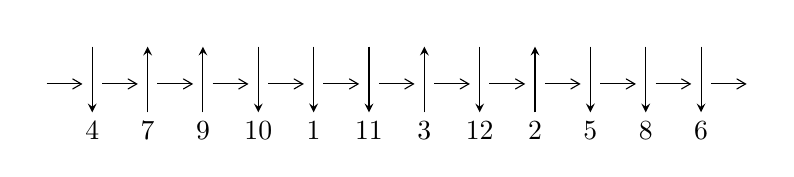
\begin{tikzpicture}[x=20pt, y=17pt]
	% nodes
	\node (C0) at (0, 0) {};
	\node (C1) at (1, 0) {};
	\node (C1U) at (1, +1) {};
	\node (C1D) at (1, -1) {4};

	\node (C2) at (2, 0) {};
	\node (C2U) at (2, +1) {};
	\node (C2D) at (2, -1) {7};

	\node (C3) at (3, 0) {};
	\node (C3U) at (3, +1) {};
	\node (C3D) at (3, -1) {9};

	\node (C4) at (4, 0) {};
	\node (C4U) at (4, +1) {};
	\node (C4D) at (4, -1) {10};

	\node (C5) at (5, 0) {};
	\node (C5U) at (5, +1) {};
	\node (C5D) at (5, -1) {1};

	\node (C6) at (6, 0) {};
	\node (C6U) at (6, +1) {};
	\node (C6D) at (6, -1) {11};

	\node (C7) at (7, 0) {};
	\node (C7U) at (7, +1) {};
	\node (C7D) at (7, -1) {3};

	\node (C8) at (8, 0) {};
	\node (C8U) at (8, +1) {};
	\node (C8D) at (8, -1) {12};

	\node (C9) at (9, 0) {};
	\node (C9U) at (9, +1) {};
	\node (C9D) at (9, -1) {2};

	\node (C10) at (10, 0) {};
	\node (C10U) at (10, +1) {};
	\node (C10D) at (10, -1) {5};

	\node (C11) at (11, 0) {};
	\node (C11U) at (11, +1) {};
	\node (C11D) at (11, -1) {8};

	\node (C12) at (12, 0) {};
	\node (C12U) at (12, +1) {};
	\node (C12D) at (12, -1) {6};
	\node (C13) at (13, 0) {};

	% arrows
	\draw[->,>={angle 60}]
	(C0) edge (C1) (C1) edge (C2) (C2) edge (C3) (C3) edge (C4) (C4) edge (C5) (C5) edge (C6) (C6) edge (C7) (C7) edge (C8) (C8) edge (C9) (C9) edge (C10) (C10) edge (C11) (C11) edge (C12) (C12) edge (C13) ;	\draw[->,>=stealth]
	(C1U) edge (C1D) (C2D) edge (C2U) (C3D) edge (C3U) (C4U) edge (C4D) (C5U) edge (C5D) (C6U) edge (C6D) (C7D) edge (C7U) (C8U) edge (C8D) (C9D) edge (C9U) (C10U) edge (C10D) (C11U) edge (C11D) (C12U) edge (C12D) ;
	\end{tikzpicture} \\
\hhline{~~} \\& 
\textbf{Solving Sequence} \\ \cline{2-2} 
 &
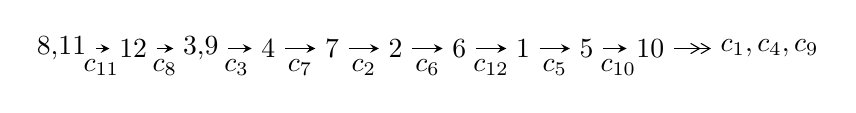
\begin{tikzpicture}[x=23pt, y=7pt]
	% node
	\node (A0) at (-1/8, 0) {8,11};
	\node (A1) at (1, 0) {12};
	\node (A2) at (33/16, 0) {3,9};
	\node (A3) at (25/8, 0) {4};
	\node (A4) at (33/8, 0) {7};
	\node (A5) at (41/8, 0) {2};
	\node (A6) at (49/8, 0) {6};
	\node (A7) at (57/8, 0) {1};
	\node (A8) at (65/8, 0) {5};
	\node (A9) at (73/8, 0) {10};
	\node (C1) at (1/2, -1) {$c_{11}$};
	\node (C2) at (3/2, -1) {$c_{8}$};
	\node (C3) at (21/8, -1) {$c_{3}$};
	\node (C4) at (29/8, -1) {$c_{7}$};
	\node (C5) at (37/8, -1) {$c_{2}$};
	\node (C6) at (45/8, -1) {$c_{6}$};
	\node (C7) at (53/8, -1) {$c_{12}$};
	\node (C8) at (61/8, -1) {$c_{5}$};
	\node (C9) at (69/8, -1) {$c_{10}$};
	\node (A10) at (11, 0) {$c_{1},c_{4},c_{9}$};

	% edge
	\draw[->,>=stealth]	
	(A0) edge (A1) (A1) edge (A2) (A2) edge (A3) (A3) edge (A4) (A4) edge (A5) (A5) edge (A6) (A6) edge (A7) (A7) edge (A8) (A8) edge (A9) ;
	\draw[->>,>={angle 60}]	
	(A9) edge (A10);
\end{tikzpicture} \\ 

\end{tabular} \\

\footnotetext{
The image of knot diagram is generated by the software ``\textbf{Draw programme}" developed by Andrew Bartholomew(\url{http://www.layer8.co.uk/maths/draw/index.htm\#Running-draw}), where we modified some parts for our purpose(\url{https://github.com/CATsTAILs/LinksPainter}).
}\phantom \\ \newline 
\centering \textbf{Ideals for irreducible components\footnotemark of $X_{\text{par}}$} 
 
\begin{align*}
I^u_{1}&=\langle 
-2.20589\times10^{861} u^{169}-1.68317\times10^{862} u^{168}+\cdots+3.92119\times10^{861} b-1.07359\times10^{864},\\
\phantom{I^u_{1}}&\phantom{= \langle  }-2.08380\times10^{863} u^{169}-1.48692\times10^{864} u^{168}+\cdots+8.66583\times10^{863} a-5.10383\times10^{865},\\
\phantom{I^u_{1}}&\phantom{= \langle  }u^{170}+8 u^{169}+\cdots-715 u+221\rangle \\
I^u_{2}&=\langle 
2.87441\times10^{31} u^{46}+1.04633\times10^{32} u^{45}+\cdots+3.67466\times10^{29} b-6.08288\times10^{31},\\
\phantom{I^u_{2}}&\phantom{= \langle  }1.01354\times10^{31} u^{46}+3.82828\times10^{31} u^{45}+\cdots+3.67466\times10^{29} a-1.99417\times10^{31},\;u^{47}+3 u^{46}+\cdots- u+1\rangle \\
\\
\end{align*}
\raggedright * 2 irreducible components of $\dim_{\mathbb{C}}=0$, with total 217 representations.\\
\footnotetext{All coefficients of polynomials are rational numbers. But the coefficients are sometimes approximated in decimal forms when there is not enough margin.}
\newpage
\renewcommand{\arraystretch}{1}
\centering \section*{I. $I^u_{1}= \langle -2.21\times10^{861} u^{169}-1.68\times10^{862} u^{168}+\cdots+3.92\times10^{861} b-1.07\times10^{864},\;-2.08\times10^{863} u^{169}-1.49\times10^{864} u^{168}+\cdots+8.67\times10^{863} a-5.10\times10^{865},\;u^{170}+8 u^{169}+\cdots-715 u+221 \rangle$}
\flushleft \textbf{(i) Arc colorings}\\
\begin{tabular}{m{7pt} m{180pt} m{7pt} m{180pt} }
\flushright $a_{8}=$&$\begin{pmatrix}0\\u\end{pmatrix}$ \\
\flushright $a_{11}=$&$\begin{pmatrix}1\\0\end{pmatrix}$ \\
\flushright $a_{12}=$&$\begin{pmatrix}1\\u^2\end{pmatrix}$ \\
\flushright $a_{3}=$&$\begin{pmatrix}0.240462 u^{169}+1.71584 u^{168}+\cdots-213.145 u+58.8960\\0.562557 u^{169}+4.29249 u^{168}+\cdots-1443.71 u+273.792\end{pmatrix}$ \\
\flushright $a_{9}=$&$\begin{pmatrix}- u\\- u^3+u\end{pmatrix}$ \\
\flushright $a_{4}=$&$\begin{pmatrix}0.345473 u^{169}+2.53056 u^{168}+\cdots-549.544 u+119.828\\0.451916 u^{169}+3.44659 u^{168}+\cdots-1148.66 u+218.467\end{pmatrix}$ \\
\flushright $a_{7}=$&$\begin{pmatrix}0.0758536 u^{169}+0.482857 u^{168}+\cdots+31.9502 u+1.29112\\0.0670230 u^{169}+0.611089 u^{168}+\cdots-518.273 u+88.7818\end{pmatrix}$ \\
\flushright $a_{2}=$&$\begin{pmatrix}1.29316 u^{169}+9.38618 u^{168}+\cdots-1589.87 u+368.013\\0.647019 u^{169}+4.85787 u^{168}+\cdots-1368.07 u+269.970\end{pmatrix}$ \\
\flushright $a_{6}=$&$\begin{pmatrix}0.142877 u^{169}+1.09395 u^{168}+\cdots-486.322 u+90.0730\\0.0670230 u^{169}+0.611089 u^{168}+\cdots-518.273 u+88.7818\end{pmatrix}$ \\
\flushright $a_{1}=$&$\begin{pmatrix}3.05118 u^{169}+22.3493 u^{168}+\cdots-4601.86 u+988.759\\1.73028 u^{169}+12.7494 u^{168}+\cdots-2868.52 u+600.253\end{pmatrix}$ \\
\flushright $a_{5}=$&$\begin{pmatrix}0.317412 u^{169}+2.17686 u^{168}+\cdots-245.983 u+62.9293\\-1.04715 u^{169}-7.63752 u^{168}+\cdots+1595.46 u-335.601\end{pmatrix}$ \\
\flushright $a_{10}=$&$\begin{pmatrix}-0.896039 u^{169}-6.43983 u^{168}+\cdots+1252.55 u-271.632\\-0.841413 u^{169}-6.23424 u^{168}+\cdots+1470.83 u-307.080\end{pmatrix}$\\&\end{tabular}
\flushleft \textbf{(ii) Obstruction class $= -1$}\\~\\
\flushleft \textbf{(iii) Cusp Shapes $= -0.513757 u^{169}-3.30789 u^{168}+\cdots-410.609 u+24.5051$}\\~\\
\newpage\renewcommand{\arraystretch}{1}
\flushleft \textbf{(iv) u-Polynomials at the component}\newline \\
\begin{tabular}{m{50pt}|m{274pt}}
Crossings & \hspace{64pt}u-Polynomials at each crossing \\
\hline $$\begin{aligned}c_{1}\end{aligned}$$&$\begin{aligned}
&u^{170}-14 u^{169}+\cdots+18 u-1
\end{aligned}$\\
\hline $$\begin{aligned}c_{2},c_{7}\end{aligned}$$&$\begin{aligned}
&u^{170}+u^{169}+\cdots-42944 u+1984
\end{aligned}$\\
\hline $$\begin{aligned}c_{3}\end{aligned}$$&$\begin{aligned}
&u^{170}- u^{169}+\cdots-276535005 u-23926117
\end{aligned}$\\
\hline $$\begin{aligned}c_{4},c_{10}\end{aligned}$$&$\begin{aligned}
&u^{170}+u^{169}+\cdots+60040 u-6379
\end{aligned}$\\
\hline $$\begin{aligned}c_{5},c_{12}\end{aligned}$$&$\begin{aligned}
&u^{170}+2 u^{169}+\cdots+6420 u-35591
\end{aligned}$\\
\hline $$\begin{aligned}c_{6}\end{aligned}$$&$\begin{aligned}
&u^{170}- u^{169}+\cdots+9130974 u+5572759
\end{aligned}$\\
\hline $$\begin{aligned}c_{8},c_{11}\end{aligned}$$&$\begin{aligned}
&u^{170}+8 u^{169}+\cdots-715 u+221
\end{aligned}$\\
\hline $$\begin{aligned}c_{9}\end{aligned}$$&$\begin{aligned}
&u^{170}+3 u^{169}+\cdots+811454 u+271819
\end{aligned}$\\
\hline
\end{tabular}\\~\\
\newpage\renewcommand{\arraystretch}{1}
\flushleft \textbf{(v) Riley Polynomials at the component}\newline \\
\begin{tabular}{m{50pt}|m{274pt}}
Crossings & \hspace{64pt}Riley Polynomials at each crossing \\
\hline $$\begin{aligned}c_{1}\end{aligned}$$&$\begin{aligned}
&y^{170}+6 y^{169}+\cdots-760 y+1
\end{aligned}$\\
\hline $$\begin{aligned}c_{2},c_{7}\end{aligned}$$&$\begin{aligned}
&y^{170}-93 y^{169}+\cdots-827236352 y+3936256
\end{aligned}$\\
\hline $$\begin{aligned}c_{3}\end{aligned}$$&$\begin{aligned}
&y^{170}-41 y^{169}+\cdots-46800698030178335 y+572459074697689
\end{aligned}$\\
\hline $$\begin{aligned}c_{4},c_{10}\end{aligned}$$&$\begin{aligned}
&y^{170}-113 y^{169}+\cdots-1618495822 y+40691641
\end{aligned}$\\
\hline $$\begin{aligned}c_{5},c_{12}\end{aligned}$$&$\begin{aligned}
&y^{170}+118 y^{169}+\cdots+25027873906 y+1266719281
\end{aligned}$\\
\hline $$\begin{aligned}c_{6}\end{aligned}$$&$\begin{aligned}
&y^{170}-9 y^{169}+\cdots+1788240547802984 y+31055642872081
\end{aligned}$\\
\hline $$\begin{aligned}c_{8},c_{11}\end{aligned}$$&$\begin{aligned}
&y^{170}-88 y^{169}+\cdots+1304511 y+48841
\end{aligned}$\\
\hline $$\begin{aligned}c_{9}\end{aligned}$$&$\begin{aligned}
&y^{170}+43 y^{169}+\cdots+6707969409918 y+73885568761
\end{aligned}$\\
\hline
\end{tabular}\\~\\
\newpage\flushleft \textbf{(vi) Complex Volumes and Cusp Shapes}
$$\begin{array}{c|c|c}  
\text{Solutions to }I^u_{1}& \I (\text{vol} + \sqrt{-1}CS) & \text{Cusp shape}\\
 \hline 
\begin{aligned}
u &= \phantom{-}0.806491 + 0.602217 I \\
a &= -0.642128 + 0.983618 I \\
b &= \phantom{-}0.19143 - 1.76020 I\end{aligned}
 & \phantom{-}7.48922 - 0.81335 I & \phantom{-0.000000 } 0 \\ \hline\begin{aligned}
u &= \phantom{-}0.806491 - 0.602217 I \\
a &= -0.642128 - 0.983618 I \\
b &= \phantom{-}0.19143 + 1.76020 I\end{aligned}
 & \phantom{-}7.48922 + 0.81335 I & \phantom{-0.000000 } 0 \\ \hline\begin{aligned}
u &= -0.923484 + 0.347149 I \\
a &= \phantom{-}1.12852 - 1.00215 I \\
b &= -0.674725 + 0.109848 I\end{aligned}
 & -5.16258 - 1.55018 I & \phantom{-0.000000 } 0 \\ \hline\begin{aligned}
u &= -0.923484 - 0.347149 I \\
a &= \phantom{-}1.12852 + 1.00215 I \\
b &= -0.674725 - 0.109848 I\end{aligned}
 & -5.16258 + 1.55018 I & \phantom{-0.000000 } 0 \\ \hline\begin{aligned}
u &= \phantom{-}0.141671 + 0.976038 I \\
a &= -0.488385 + 1.125170 I \\
b &= -0.03831 - 1.42440 I\end{aligned}
 & \phantom{-}3.36613 + 3.99327 I & \phantom{-0.000000 } 0 \\ \hline\begin{aligned}
u &= \phantom{-}0.141671 - 0.976038 I \\
a &= -0.488385 - 1.125170 I \\
b &= -0.03831 + 1.42440 I\end{aligned}
 & \phantom{-}3.36613 - 3.99327 I & \phantom{-0.000000 } 0 \\ \hline\begin{aligned}
u &= \phantom{-}0.956886 + 0.364577 I \\
a &= \phantom{-}1.035210 - 0.734016 I \\
b &= -0.30003 + 2.40004 I\end{aligned}
 & \phantom{-}2.92615 - 8.39267 I & \phantom{-0.000000 } 0 \\ \hline\begin{aligned}
u &= \phantom{-}0.956886 - 0.364577 I \\
a &= \phantom{-}1.035210 + 0.734016 I \\
b &= -0.30003 - 2.40004 I\end{aligned}
 & \phantom{-}2.92615 + 8.39267 I & \phantom{-0.000000 } 0 \\ \hline\begin{aligned}
u &= \phantom{-}0.798269 + 0.554483 I \\
a &= -1.29539 + 0.66106 I \\
b &= -0.907230 - 0.822265 I\end{aligned}
 & \phantom{-}7.53091 - 3.76031 I & \phantom{-0.000000 } 0 \\ \hline\begin{aligned}
u &= \phantom{-}0.798269 - 0.554483 I \\
a &= -1.29539 - 0.66106 I \\
b &= -0.907230 + 0.822265 I\end{aligned}
 & \phantom{-}7.53091 + 3.76031 I & \phantom{-0.000000 } 0\\
 \hline 
 \end{array}$$\newpage$$\begin{array}{c|c|c}  
\text{Solutions to }I^u_{1}& \I (\text{vol} + \sqrt{-1}CS) & \text{Cusp shape}\\
 \hline 
\begin{aligned}
u &= -0.831602 + 0.494310 I \\
a &= -1.48201 - 0.73010 I \\
b &= -0.840353 + 1.057020 I\end{aligned}
 & \phantom{-}4.31538 + 8.41906 I & \phantom{-0.000000 } 0 \\ \hline\begin{aligned}
u &= -0.831602 - 0.494310 I \\
a &= -1.48201 + 0.73010 I \\
b &= -0.840353 - 1.057020 I\end{aligned}
 & \phantom{-}4.31538 - 8.41906 I & \phantom{-0.000000 } 0 \\ \hline\begin{aligned}
u &= -0.338787 + 0.978329 I \\
a &= -0.007267 - 0.513671 I \\
b &= -0.80769 + 1.41151 I\end{aligned}
 & \phantom{-}3.70858 + 2.48023 I & \phantom{-0.000000 } 0 \\ \hline\begin{aligned}
u &= -0.338787 - 0.978329 I \\
a &= -0.007267 + 0.513671 I \\
b &= -0.80769 - 1.41151 I\end{aligned}
 & \phantom{-}3.70858 - 2.48023 I & \phantom{-0.000000 } 0 \\ \hline\begin{aligned}
u &= -0.802710 + 0.530461 I \\
a &= -0.947896 - 1.022750 I \\
b &= \phantom{-}0.15648 + 1.76490 I\end{aligned}
 & \phantom{-}4.38227 - 4.26234 I & \phantom{-0.000000 } 0 \\ \hline\begin{aligned}
u &= -0.802710 - 0.530461 I \\
a &= -0.947896 + 1.022750 I \\
b &= \phantom{-}0.15648 - 1.76490 I\end{aligned}
 & \phantom{-}4.38227 + 4.26234 I & \phantom{-0.000000 } 0 \\ \hline\begin{aligned}
u &= -1.044890 + 0.163904 I \\
a &= -0.738916 - 0.484622 I \\
b &= -0.99773 + 1.59669 I\end{aligned}
 & -1.66846 + 0.48444 I & \phantom{-0.000000 } 0 \\ \hline\begin{aligned}
u &= -1.044890 - 0.163904 I \\
a &= -0.738916 + 0.484622 I \\
b &= -0.99773 - 1.59669 I\end{aligned}
 & -1.66846 - 0.48444 I & \phantom{-0.000000 } 0 \\ \hline\begin{aligned}
u &= -0.414758 + 0.845908 I \\
a &= \phantom{-}0.183797 - 1.029530 I \\
b &= \phantom{-}0.40704 + 1.83699 I\end{aligned}
 & \phantom{-}0.96077 + 6.50241 I & \phantom{-0.000000 } 0 \\ \hline\begin{aligned}
u &= -0.414758 - 0.845908 I \\
a &= \phantom{-}0.183797 + 1.029530 I \\
b &= \phantom{-}0.40704 - 1.83699 I\end{aligned}
 & \phantom{-}0.96077 - 6.50241 I & \phantom{-0.000000 } 0\\
 \hline 
 \end{array}$$\newpage$$\begin{array}{c|c|c}  
\text{Solutions to }I^u_{1}& \I (\text{vol} + \sqrt{-1}CS) & \text{Cusp shape}\\
 \hline 
\begin{aligned}
u &= -0.158664 + 1.046010 I \\
a &= -0.605569 - 1.030360 I \\
b &= \phantom{-}0.236176 + 1.351120 I\end{aligned}
 & -0.85216 - 7.75918 I & \phantom{-0.000000 } 0 \\ \hline\begin{aligned}
u &= -0.158664 - 1.046010 I \\
a &= -0.605569 + 1.030360 I \\
b &= \phantom{-}0.236176 - 1.351120 I\end{aligned}
 & -0.85216 + 7.75918 I & \phantom{-0.000000 } 0 \\ \hline\begin{aligned}
u &= \phantom{-}0.834299 + 0.650852 I \\
a &= -0.098909 + 1.187020 I \\
b &= -1.35369 - 1.59644 I\end{aligned}
 & -3.52491 - 5.82721 I & \phantom{-0.000000 } 0 \\ \hline\begin{aligned}
u &= \phantom{-}0.834299 - 0.650852 I \\
a &= -0.098909 - 1.187020 I \\
b &= -1.35369 + 1.59644 I\end{aligned}
 & -3.52491 + 5.82721 I & \phantom{-0.000000 } 0 \\ \hline\begin{aligned}
u &= -1.018280 + 0.313229 I \\
a &= \phantom{-}0.828726 + 0.572675 I \\
b &= -1.02081 - 1.92324 I\end{aligned}
 & \phantom{-}4.88864 + 3.76517 I & \phantom{-0.000000 } 0 \\ \hline\begin{aligned}
u &= -1.018280 - 0.313229 I \\
a &= \phantom{-}0.828726 - 0.572675 I \\
b &= -1.02081 + 1.92324 I\end{aligned}
 & \phantom{-}4.88864 - 3.76517 I & \phantom{-0.000000 } 0 \\ \hline\begin{aligned}
u &= \phantom{-}0.224394 + 0.906655 I \\
a &= -0.559436 - 0.349460 I \\
b &= \phantom{-}0.096076 + 0.954016 I\end{aligned}
 & \phantom{-}4.22731 + 2.52538 I & \phantom{-0.000000 } 0 \\ \hline\begin{aligned}
u &= \phantom{-}0.224394 - 0.906655 I \\
a &= -0.559436 + 0.349460 I \\
b &= \phantom{-}0.096076 - 0.954016 I\end{aligned}
 & \phantom{-}4.22731 - 2.52538 I & \phantom{-0.000000 } 0 \\ \hline\begin{aligned}
u &= \phantom{-}1.036580 + 0.282285 I \\
a &= -0.811496 + 0.728701 I \\
b &= -1.43074 - 1.60823 I\end{aligned}
 & -6.33389 - 5.42778 I & \phantom{-0.000000 } 0 \\ \hline\begin{aligned}
u &= \phantom{-}1.036580 - 0.282285 I \\
a &= -0.811496 - 0.728701 I \\
b &= -1.43074 + 1.60823 I\end{aligned}
 & -6.33389 + 5.42778 I & \phantom{-0.000000 } 0\\
 \hline 
 \end{array}$$\newpage$$\begin{array}{c|c|c}  
\text{Solutions to }I^u_{1}& \I (\text{vol} + \sqrt{-1}CS) & \text{Cusp shape}\\
 \hline 
\begin{aligned}
u &= -0.366311 + 1.028260 I \\
a &= -0.601079 - 0.608587 I \\
b &= -0.376946 + 0.702967 I\end{aligned}
 & \phantom{-}1.11850 + 2.49775 I & \phantom{-0.000000 } 0 \\ \hline\begin{aligned}
u &= -0.366311 - 1.028260 I \\
a &= -0.601079 + 0.608587 I \\
b &= -0.376946 - 0.702967 I\end{aligned}
 & \phantom{-}1.11850 - 2.49775 I & \phantom{-0.000000 } 0 \\ \hline\begin{aligned}
u &= \phantom{-}0.955413 + 0.535542 I \\
a &= -1.031710 - 0.527843 I \\
b &= \phantom{-}0.492943 - 0.739556 I\end{aligned}
 & -4.00039 + 1.13083 I & \phantom{-0.000000 } 0 \\ \hline\begin{aligned}
u &= \phantom{-}0.955413 - 0.535542 I \\
a &= -1.031710 + 0.527843 I \\
b &= \phantom{-}0.492943 + 0.739556 I\end{aligned}
 & -4.00039 - 1.13083 I & \phantom{-0.000000 } 0 \\ \hline\begin{aligned}
u &= \phantom{-}1.085970 + 0.244696 I \\
a &= \phantom{-}0.996060 + 0.557928 I \\
b &= -0.051939 + 0.187299 I\end{aligned}
 & -2.66025 + 2.54993 I & \phantom{-0.000000 } 0 \\ \hline\begin{aligned}
u &= \phantom{-}1.085970 - 0.244696 I \\
a &= \phantom{-}0.996060 - 0.557928 I \\
b &= -0.051939 - 0.187299 I\end{aligned}
 & -2.66025 - 2.54993 I & \phantom{-0.000000 } 0 \\ \hline\begin{aligned}
u &= \phantom{-}0.874696 + 0.133073 I \\
a &= \phantom{-}0.774374 + 1.094520 I \\
b &= -0.046872 - 0.469309 I\end{aligned}
 & -1.30487 + 1.72427 I & \phantom{-0.000000 } 0 \\ \hline\begin{aligned}
u &= \phantom{-}0.874696 - 0.133073 I \\
a &= \phantom{-}0.774374 - 1.094520 I \\
b &= -0.046872 + 0.469309 I\end{aligned}
 & -1.30487 - 1.72427 I & \phantom{-0.000000 } 0 \\ \hline\begin{aligned}
u &= -0.497941 + 0.729795 I \\
a &= \phantom{-}1.165820 + 0.629819 I \\
b &= \phantom{-}0.006520 - 0.998511 I\end{aligned}
 & -2.03235 - 1.15583 I & \phantom{-0.000000 } 0 \\ \hline\begin{aligned}
u &= -0.497941 - 0.729795 I \\
a &= \phantom{-}1.165820 - 0.629819 I \\
b &= \phantom{-}0.006520 + 0.998511 I\end{aligned}
 & -2.03235 + 1.15583 I & \phantom{-0.000000 } 0\\
 \hline 
 \end{array}$$\newpage$$\begin{array}{c|c|c}  
\text{Solutions to }I^u_{1}& \I (\text{vol} + \sqrt{-1}CS) & \text{Cusp shape}\\
 \hline 
\begin{aligned}
u &= \phantom{-}1.061980 + 0.362119 I \\
a &= -0.528626 - 0.797838 I \\
b &= \phantom{-}0.149722 + 0.444329 I\end{aligned}
 & -2.90057 - 3.69809 I & \phantom{-0.000000 } 0 \\ \hline\begin{aligned}
u &= \phantom{-}1.061980 - 0.362119 I \\
a &= -0.528626 + 0.797838 I \\
b &= \phantom{-}0.149722 - 0.444329 I\end{aligned}
 & -2.90057 + 3.69809 I & \phantom{-0.000000 } 0 \\ \hline\begin{aligned}
u &= -1.002390 + 0.507253 I \\
a &= -0.775875 - 0.405924 I \\
b &= \phantom{-}0.36366 + 1.97753 I\end{aligned}
 & \phantom{-}2.66744 + 2.88124 I & \phantom{-0.000000 } 0 \\ \hline\begin{aligned}
u &= -1.002390 - 0.507253 I \\
a &= -0.775875 + 0.405924 I \\
b &= \phantom{-}0.36366 - 1.97753 I\end{aligned}
 & \phantom{-}2.66744 - 2.88124 I & \phantom{-0.000000 } 0 \\ \hline\begin{aligned}
u &= \phantom{-}1.039130 + 0.442035 I \\
a &= -0.012302 - 0.813686 I \\
b &= \phantom{-}0.719743 + 1.063800 I\end{aligned}
 & -4.03539 - 3.56778 I & \phantom{-0.000000 } 0 \\ \hline\begin{aligned}
u &= \phantom{-}1.039130 - 0.442035 I \\
a &= -0.012302 + 0.813686 I \\
b &= \phantom{-}0.719743 - 1.063800 I\end{aligned}
 & -4.03539 + 3.56778 I & \phantom{-0.000000 } 0 \\ \hline\begin{aligned}
u &= -1.090030 + 0.319356 I \\
a &= -0.276890 + 0.948683 I \\
b &= \phantom{-}0.701189 - 0.427324 I\end{aligned}
 & -4.85761 + 3.45164 I & \phantom{-0.000000 } 0 \\ \hline\begin{aligned}
u &= -1.090030 - 0.319356 I \\
a &= -0.276890 - 0.948683 I \\
b &= \phantom{-}0.701189 + 0.427324 I\end{aligned}
 & -4.85761 - 3.45164 I & \phantom{-0.000000 } 0 \\ \hline\begin{aligned}
u &= -1.078490 + 0.389234 I \\
a &= -0.787230 + 0.880471 I \\
b &= \phantom{-}0.048133 - 0.220752 I\end{aligned}
 & -6.77478 + 6.50412 I & \phantom{-0.000000 } 0 \\ \hline\begin{aligned}
u &= -1.078490 - 0.389234 I \\
a &= -0.787230 - 0.880471 I \\
b &= \phantom{-}0.048133 + 0.220752 I\end{aligned}
 & -6.77478 - 6.50412 I & \phantom{-0.000000 } 0\\
 \hline 
 \end{array}$$\newpage$$\begin{array}{c|c|c}  
\text{Solutions to }I^u_{1}& \I (\text{vol} + \sqrt{-1}CS) & \text{Cusp shape}\\
 \hline 
\begin{aligned}
u &= -0.264729 + 0.810062 I \\
a &= -0.919199 + 0.505820 I \\
b &= \phantom{-}0.468141 - 0.933035 I\end{aligned}
 & -0.28815 - 8.54272 I & \phantom{-0.000000 } 0 \\ \hline\begin{aligned}
u &= -0.264729 - 0.810062 I \\
a &= -0.919199 - 0.505820 I \\
b &= \phantom{-}0.468141 + 0.933035 I\end{aligned}
 & -0.28815 + 8.54272 I & \phantom{-0.000000 } 0 \\ \hline\begin{aligned}
u &= \phantom{-}1.074410 + 0.405058 I \\
a &= -0.271488 - 0.968396 I \\
b &= \phantom{-}0.076752 + 0.262131 I\end{aligned}
 & -1.51684 - 6.06281 I & \phantom{-0.000000 } 0 \\ \hline\begin{aligned}
u &= \phantom{-}1.074410 - 0.405058 I \\
a &= -0.271488 + 0.968396 I \\
b &= \phantom{-}0.076752 - 0.262131 I\end{aligned}
 & -1.51684 + 6.06281 I & \phantom{-0.000000 } 0 \\ \hline\begin{aligned}
u &= \phantom{-}0.770082 + 0.363667 I \\
a &= \phantom{-}1.69569 - 0.51875 I \\
b &= \phantom{-}1.41698 + 1.21974 I\end{aligned}
 & \phantom{-}3.56946 + 5.26691 I & \phantom{-0.000000 } 0 \\ \hline\begin{aligned}
u &= \phantom{-}0.770082 - 0.363667 I \\
a &= \phantom{-}1.69569 + 0.51875 I \\
b &= \phantom{-}1.41698 - 1.21974 I\end{aligned}
 & \phantom{-}3.56946 - 5.26691 I & \phantom{-0.000000 } 0 \\ \hline\begin{aligned}
u &= -1.087010 + 0.390708 I \\
a &= \phantom{-}0.564034 + 1.103930 I \\
b &= \phantom{-}0.049728 - 0.981981 I\end{aligned}
 & \phantom{-}1.73688 + 5.19821 I & \phantom{-0.000000 } 0 \\ \hline\begin{aligned}
u &= -1.087010 - 0.390708 I \\
a &= \phantom{-}0.564034 - 1.103930 I \\
b &= \phantom{-}0.049728 + 0.981981 I\end{aligned}
 & \phantom{-}1.73688 - 5.19821 I & \phantom{-0.000000 } 0 \\ \hline\begin{aligned}
u &= -1.014070 + 0.566273 I \\
a &= \phantom{-}0.511883 + 1.128890 I \\
b &= \phantom{-}0.85240 - 1.71737 I\end{aligned}
 & -3.51186 + 6.09555 I & \phantom{-0.000000 } 0 \\ \hline\begin{aligned}
u &= -1.014070 - 0.566273 I \\
a &= \phantom{-}0.511883 - 1.128890 I \\
b &= \phantom{-}0.85240 + 1.71737 I\end{aligned}
 & -3.51186 - 6.09555 I & \phantom{-0.000000 } 0\\
 \hline 
 \end{array}$$\newpage$$\begin{array}{c|c|c}  
\text{Solutions to }I^u_{1}& \I (\text{vol} + \sqrt{-1}CS) & \text{Cusp shape}\\
 \hline 
\begin{aligned}
u &= \phantom{-}1.085820 + 0.418233 I \\
a &= \phantom{-}0.798553 - 1.006530 I \\
b &= \phantom{-}0.222149 + 1.264500 I\end{aligned}
 & \phantom{-}1.81434 - 3.63679 I & \phantom{-0.000000 } 0 \\ \hline\begin{aligned}
u &= \phantom{-}1.085820 - 0.418233 I \\
a &= \phantom{-}0.798553 + 1.006530 I \\
b &= \phantom{-}0.222149 - 1.264500 I\end{aligned}
 & \phantom{-}1.81434 + 3.63679 I & \phantom{-0.000000 } 0 \\ \hline\begin{aligned}
u &= \phantom{-}1.032740 + 0.540789 I \\
a &= -0.639624 + 0.255097 I \\
b &= \phantom{-}0.64336 - 1.81774 I\end{aligned}
 & \phantom{-}3.05780 - 1.58165 I & \phantom{-0.000000 } 0 \\ \hline\begin{aligned}
u &= \phantom{-}1.032740 - 0.540789 I \\
a &= -0.639624 - 0.255097 I \\
b &= \phantom{-}0.64336 + 1.81774 I\end{aligned}
 & \phantom{-}3.05780 + 1.58165 I & \phantom{-0.000000 } 0 \\ \hline\begin{aligned}
u &= -1.172030 + 0.110315 I \\
a &= \phantom{-}0.546361 - 0.282163 I \\
b &= \phantom{-}0.338652 - 0.023447 I\end{aligned}
 & -1.85244 - 0.13124 I & \phantom{-0.000000 } 0 \\ \hline\begin{aligned}
u &= -1.172030 - 0.110315 I \\
a &= \phantom{-}0.546361 + 0.282163 I \\
b &= \phantom{-}0.338652 + 0.023447 I\end{aligned}
 & -1.85244 + 0.13124 I & \phantom{-0.000000 } 0 \\ \hline\begin{aligned}
u &= \phantom{-}0.206943 + 0.792165 I \\
a &= -0.77995 + 1.43503 I \\
b &= -0.23213 - 1.55337 I\end{aligned}
 & \phantom{-}3.35332 + 3.66686 I & \phantom{-0.000000 } 0 \\ \hline\begin{aligned}
u &= \phantom{-}0.206943 - 0.792165 I \\
a &= -0.77995 - 1.43503 I \\
b &= -0.23213 + 1.55337 I\end{aligned}
 & \phantom{-}3.35332 - 3.66686 I & \phantom{-0.000000 } 0 \\ \hline\begin{aligned}
u &= \phantom{-}1.073230 + 0.497941 I \\
a &= \phantom{-}0.718078 - 0.898766 I \\
b &= \phantom{-}0.56627 + 1.47951 I\end{aligned}
 & \phantom{-}1.19048 - 4.34256 I & \phantom{-0.000000 } 0 \\ \hline\begin{aligned}
u &= \phantom{-}1.073230 - 0.497941 I \\
a &= \phantom{-}0.718078 + 0.898766 I \\
b &= \phantom{-}0.56627 - 1.47951 I\end{aligned}
 & \phantom{-}1.19048 + 4.34256 I & \phantom{-0.000000 } 0\\
 \hline 
 \end{array}$$\newpage$$\begin{array}{c|c|c}  
\text{Solutions to }I^u_{1}& \I (\text{vol} + \sqrt{-1}CS) & \text{Cusp shape}\\
 \hline 
\begin{aligned}
u &= -0.386200 + 0.716926 I \\
a &= -1.23518 - 1.03634 I \\
b &= -0.09588 + 1.72609 I\end{aligned}
 & \phantom{-}1.62100 - 4.92629 I & \phantom{-0.000000 } 0 \\ \hline\begin{aligned}
u &= -0.386200 - 0.716926 I \\
a &= -1.23518 + 1.03634 I \\
b &= -0.09588 - 1.72609 I\end{aligned}
 & \phantom{-}1.62100 + 4.92629 I & \phantom{-0.000000 } 0 \\ \hline\begin{aligned}
u &= -1.087760 + 0.478529 I \\
a &= -0.398562 + 0.536807 I \\
b &= -0.090742 + 0.198724 I\end{aligned}
 & \phantom{-}1.11222 + 2.21408 I & \phantom{-0.000000 } 0 \\ \hline\begin{aligned}
u &= -1.087760 - 0.478529 I \\
a &= -0.398562 - 0.536807 I \\
b &= -0.090742 - 0.198724 I\end{aligned}
 & \phantom{-}1.11222 - 2.21408 I & \phantom{-0.000000 } 0 \\ \hline\begin{aligned}
u &= \phantom{-}0.720394 + 0.363656 I \\
a &= \phantom{-}0.1003940 - 0.0876140 I \\
b &= \phantom{-}0.09773 + 1.62111 I\end{aligned}
 & -4.26294 - 3.88455 I & \phantom{-0.000000 } 0 \\ \hline\begin{aligned}
u &= \phantom{-}0.720394 - 0.363656 I \\
a &= \phantom{-}0.1003940 + 0.0876140 I \\
b &= \phantom{-}0.09773 - 1.62111 I\end{aligned}
 & -4.26294 + 3.88455 I & \phantom{-0.000000 } 0 \\ \hline\begin{aligned}
u &= -0.751811 + 0.261150 I \\
a &= \phantom{-}1.67265 + 0.26483 I \\
b &= \phantom{-}1.79961 - 0.35379 I\end{aligned}
 & \phantom{-}5.89546 - 1.20354 I & \phantom{-0.000000 } 0 \\ \hline\begin{aligned}
u &= -0.751811 - 0.261150 I \\
a &= \phantom{-}1.67265 - 0.26483 I \\
b &= \phantom{-}1.79961 + 0.35379 I\end{aligned}
 & \phantom{-}5.89546 + 1.20354 I & \phantom{-0.000000 } 0 \\ \hline\begin{aligned}
u &= \phantom{-}1.077970 + 0.559514 I \\
a &= \phantom{-}0.528140 - 0.647463 I \\
b &= \phantom{-}1.59630 + 1.38440 I\end{aligned}
 & -5.68088 - 0.47001 I & \phantom{-0.000000 } 0 \\ \hline\begin{aligned}
u &= \phantom{-}1.077970 - 0.559514 I \\
a &= \phantom{-}0.528140 + 0.647463 I \\
b &= \phantom{-}1.59630 - 1.38440 I\end{aligned}
 & -5.68088 + 0.47001 I & \phantom{-0.000000 } 0\\
 \hline 
 \end{array}$$\newpage$$\begin{array}{c|c|c}  
\text{Solutions to }I^u_{1}& \I (\text{vol} + \sqrt{-1}CS) & \text{Cusp shape}\\
 \hline 
\begin{aligned}
u &= \phantom{-}1.141460 + 0.436982 I \\
a &= \phantom{-}0.719505 - 0.582562 I \\
b &= \phantom{-}1.79355 + 2.15528 I\end{aligned}
 & -2.77969 - 9.91991 I & \phantom{-0.000000 } 0 \\ \hline\begin{aligned}
u &= \phantom{-}1.141460 - 0.436982 I \\
a &= \phantom{-}0.719505 + 0.582562 I \\
b &= \phantom{-}1.79355 - 2.15528 I\end{aligned}
 & -2.77969 + 9.91991 I & \phantom{-0.000000 } 0 \\ \hline\begin{aligned}
u &= -0.412691 + 1.159020 I \\
a &= \phantom{-}0.751366 + 0.779719 I \\
b &= \phantom{-}0.13006 - 1.68933 I\end{aligned}
 & \phantom{-}2.83336 - 13.74430 I & \phantom{-0.000000 } 0 \\ \hline\begin{aligned}
u &= -0.412691 - 1.159020 I \\
a &= \phantom{-}0.751366 - 0.779719 I \\
b &= \phantom{-}0.13006 + 1.68933 I\end{aligned}
 & \phantom{-}2.83336 + 13.74430 I & \phantom{-0.000000 } 0 \\ \hline\begin{aligned}
u &= -0.759159 + 0.077930 I \\
a &= \phantom{-}0.27620 + 1.61746 I \\
b &= \phantom{-}0.358040 - 0.701749 I\end{aligned}
 & -4.43746 + 4.02048 I & \phantom{-0.000000 } 0 \\ \hline\begin{aligned}
u &= -0.759159 - 0.077930 I \\
a &= \phantom{-}0.27620 - 1.61746 I \\
b &= \phantom{-}0.358040 + 0.701749 I\end{aligned}
 & -4.43746 - 4.02048 I & \phantom{-0.000000 } 0 \\ \hline\begin{aligned}
u &= \phantom{-}1.218450 + 0.215306 I \\
a &= -0.492939 + 0.554272 I \\
b &= -1.21497 - 1.07752 I\end{aligned}
 & -5.11241 + 5.14848 I & \phantom{-0.000000 } 0 \\ \hline\begin{aligned}
u &= \phantom{-}1.218450 - 0.215306 I \\
a &= -0.492939 - 0.554272 I \\
b &= -1.21497 + 1.07752 I\end{aligned}
 & -5.11241 - 5.14848 I & \phantom{-0.000000 } 0 \\ \hline\begin{aligned}
u &= -1.103990 + 0.569699 I \\
a &= -0.767471 - 0.982847 I \\
b &= -1.20004 + 2.17363 I\end{aligned}
 & -0.49000 + 9.86610 I & \phantom{-0.000000 } 0 \\ \hline\begin{aligned}
u &= -1.103990 - 0.569699 I \\
a &= -0.767471 + 0.982847 I \\
b &= -1.20004 - 2.17363 I\end{aligned}
 & -0.49000 - 9.86610 I & \phantom{-0.000000 } 0\\
 \hline 
 \end{array}$$\newpage$$\begin{array}{c|c|c}  
\text{Solutions to }I^u_{1}& \I (\text{vol} + \sqrt{-1}CS) & \text{Cusp shape}\\
 \hline 
\begin{aligned}
u &= \phantom{-}0.453656 + 1.178900 I \\
a &= -0.531767 + 0.782266 I \\
b &= -0.08702 - 1.78565 I\end{aligned}
 & \phantom{-}5.39447 + 4.87671 I & \phantom{-0.000000 } 0 \\ \hline\begin{aligned}
u &= \phantom{-}0.453656 - 1.178900 I \\
a &= -0.531767 - 0.782266 I \\
b &= -0.08702 + 1.78565 I\end{aligned}
 & \phantom{-}5.39447 - 4.87671 I & \phantom{-0.000000 } 0 \\ \hline\begin{aligned}
u &= -0.730425\phantom{ +0.000000I} \\
a &= \phantom{-}0.666694\phantom{ +0.000000I} \\
b &= \phantom{-}0.382456\phantom{ +0.000000I}\end{aligned}
 & -1.46358\phantom{ +0.000000I} & \phantom{-0.000000 } 0 \\ \hline\begin{aligned}
u &= -1.086450 + 0.664366 I \\
a &= \phantom{-}0.482956 + 0.569224 I \\
b &= \phantom{-}0.96455 - 1.58617 I\end{aligned}
 & -1.16037 + 2.89712 I & \phantom{-0.000000 } 0 \\ \hline\begin{aligned}
u &= -1.086450 - 0.664366 I \\
a &= \phantom{-}0.482956 - 0.569224 I \\
b &= \phantom{-}0.96455 + 1.58617 I\end{aligned}
 & -1.16037 - 2.89712 I & \phantom{-0.000000 } 0 \\ \hline\begin{aligned}
u &= \phantom{-}0.499069 + 0.527627 I \\
a &= -0.88297 + 1.37264 I \\
b &= -1.43447 - 0.40397 I\end{aligned}
 & \phantom{-}4.65459 - 2.82623 I & \phantom{-0.000000 } 0 \\ \hline\begin{aligned}
u &= \phantom{-}0.499069 - 0.527627 I \\
a &= -0.88297 - 1.37264 I \\
b &= -1.43447 + 0.40397 I\end{aligned}
 & \phantom{-}4.65459 + 2.82623 I & \phantom{-0.000000 } 0 \\ \hline\begin{aligned}
u &= -1.161360 + 0.525226 I \\
a &= \phantom{-}0.754007 + 0.654124 I \\
b &= \phantom{-}0.688330 - 1.215040 I\end{aligned}
 & -0.390599 + 1.111860 I & \phantom{-0.000000 } 0 \\ \hline\begin{aligned}
u &= -1.161360 - 0.525226 I \\
a &= \phantom{-}0.754007 - 0.654124 I \\
b &= \phantom{-}0.688330 + 1.215040 I\end{aligned}
 & -0.390599 - 1.111860 I & \phantom{-0.000000 } 0 \\ \hline\begin{aligned}
u &= -0.608042 + 0.394118 I \\
a &= -1.44804 - 1.10655 I \\
b &= -1.46064 + 0.72845 I\end{aligned}
 & \phantom{-}3.98560 + 1.07651 I & \phantom{-0.000000 } 0\\
 \hline 
 \end{array}$$\newpage$$\begin{array}{c|c|c}  
\text{Solutions to }I^u_{1}& \I (\text{vol} + \sqrt{-1}CS) & \text{Cusp shape}\\
 \hline 
\begin{aligned}
u &= -0.608042 - 0.394118 I \\
a &= -1.44804 + 1.10655 I \\
b &= -1.46064 - 0.72845 I\end{aligned}
 & \phantom{-}3.98560 - 1.07651 I & \phantom{-0.000000 } 0 \\ \hline\begin{aligned}
u &= \phantom{-}1.151370 + 0.560793 I \\
a &= -0.779456 + 0.840590 I \\
b &= -0.89795 - 2.16549 I\end{aligned}
 & \phantom{-}0.68066 - 8.67829 I & \phantom{-0.000000 } 0 \\ \hline\begin{aligned}
u &= \phantom{-}1.151370 - 0.560793 I \\
a &= -0.779456 - 0.840590 I \\
b &= -0.89795 + 2.16549 I\end{aligned}
 & \phantom{-}0.68066 + 8.67829 I & \phantom{-0.000000 } 0 \\ \hline\begin{aligned}
u &= -1.158310 + 0.565107 I \\
a &= \phantom{-}0.651043 - 0.728404 I \\
b &= -0.379605 + 0.088246 I\end{aligned}
 & -2.91077 + 13.64960 I & \phantom{-0.000000 } 0 \\ \hline\begin{aligned}
u &= -1.158310 - 0.565107 I \\
a &= \phantom{-}0.651043 + 0.728404 I \\
b &= -0.379605 - 0.088246 I\end{aligned}
 & -2.91077 - 13.64960 I & \phantom{-0.000000 } 0 \\ \hline\begin{aligned}
u &= -0.259853 + 1.266720 I \\
a &= \phantom{-}0.080496 + 0.743006 I \\
b &= \phantom{-}0.08175 - 1.53457 I\end{aligned}
 & \phantom{-}2.98324 + 4.47610 I & \phantom{-0.000000 } 0 \\ \hline\begin{aligned}
u &= -0.259853 - 1.266720 I \\
a &= \phantom{-}0.080496 - 0.743006 I \\
b &= \phantom{-}0.08175 + 1.53457 I\end{aligned}
 & \phantom{-}2.98324 - 4.47610 I & \phantom{-0.000000 } 0 \\ \hline\begin{aligned}
u &= -0.420304 + 1.229010 I \\
a &= \phantom{-}0.408093 + 0.560897 I \\
b &= \phantom{-}0.63897 - 1.98417 I\end{aligned}
 & \phantom{-}2.83986 + 2.69706 I & \phantom{-0.000000 } 0 \\ \hline\begin{aligned}
u &= -0.420304 - 1.229010 I \\
a &= \phantom{-}0.408093 - 0.560897 I \\
b &= \phantom{-}0.63897 + 1.98417 I\end{aligned}
 & \phantom{-}2.83986 - 2.69706 I & \phantom{-0.000000 } 0 \\ \hline\begin{aligned}
u &= \phantom{-}1.308170 + 0.087102 I \\
a &= -0.422502 - 0.416698 I \\
b &= \phantom{-}0.371850 + 0.107744 I\end{aligned}
 & -7.93701 - 1.01267 I & \phantom{-0.000000 } 0\\
 \hline 
 \end{array}$$\newpage$$\begin{array}{c|c|c}  
\text{Solutions to }I^u_{1}& \I (\text{vol} + \sqrt{-1}CS) & \text{Cusp shape}\\
 \hline 
\begin{aligned}
u &= \phantom{-}1.308170 - 0.087102 I \\
a &= -0.422502 + 0.416698 I \\
b &= \phantom{-}0.371850 - 0.107744 I\end{aligned}
 & -7.93701 + 1.01267 I & \phantom{-0.000000 } 0 \\ \hline\begin{aligned}
u &= \phantom{-}1.176760 + 0.579739 I \\
a &= \phantom{-}0.569992 + 0.583963 I \\
b &= -0.188102 - 0.147284 I\end{aligned}
 & \phantom{-}1.43457 - 7.87964 I & \phantom{-0.000000 } 0 \\ \hline\begin{aligned}
u &= \phantom{-}1.176760 - 0.579739 I \\
a &= \phantom{-}0.569992 - 0.583963 I \\
b &= -0.188102 + 0.147284 I\end{aligned}
 & \phantom{-}1.43457 + 7.87964 I & \phantom{-0.000000 } 0 \\ \hline\begin{aligned}
u &= \phantom{-}0.663821 + 0.163673 I \\
a &= \phantom{-}1.47918 + 0.96656 I \\
b &= \phantom{-}0.116724 - 1.086720 I\end{aligned}
 & \phantom{-}0.37077 + 3.23302 I & \phantom{-0.000000 } 0 \\ \hline\begin{aligned}
u &= \phantom{-}0.663821 - 0.163673 I \\
a &= \phantom{-}1.47918 - 0.96656 I \\
b &= \phantom{-}0.116724 + 1.086720 I\end{aligned}
 & \phantom{-}0.37077 - 3.23302 I & \phantom{-0.000000 } 0 \\ \hline\begin{aligned}
u &= \phantom{-}0.285135 + 0.610380 I \\
a &= \phantom{-}0.92416 - 1.60790 I \\
b &= -0.050637 + 0.924680 I\end{aligned}
 & \phantom{-}3.32659 + 0.00720 I & \phantom{-0.000000 } 0 \\ \hline\begin{aligned}
u &= \phantom{-}0.285135 - 0.610380 I \\
a &= \phantom{-}0.92416 + 1.60790 I \\
b &= -0.050637 - 0.924680 I\end{aligned}
 & \phantom{-}3.32659 - 0.00720 I & \phantom{-0.000000 } 0 \\ \hline\begin{aligned}
u &= \phantom{-}0.489942 + 1.238200 I \\
a &= \phantom{-}0.662960 - 0.648185 I \\
b &= \phantom{-}0.32328 + 1.65794 I\end{aligned}
 & \phantom{-}6.77832 + 6.88044 I & \phantom{-0.000000 } 0 \\ \hline\begin{aligned}
u &= \phantom{-}0.489942 - 1.238200 I \\
a &= \phantom{-}0.662960 + 0.648185 I \\
b &= \phantom{-}0.32328 - 1.65794 I\end{aligned}
 & \phantom{-}6.77832 - 6.88044 I & \phantom{-0.000000 } 0 \\ \hline\begin{aligned}
u &= -0.224321 + 0.627904 I \\
a &= -0.015286 - 0.524588 I \\
b &= -0.697858 - 0.367055 I\end{aligned}
 & \phantom{-}1.46936 + 3.06749 I & \phantom{-0.000000 } 0\\
 \hline 
 \end{array}$$\newpage$$\begin{array}{c|c|c}  
\text{Solutions to }I^u_{1}& \I (\text{vol} + \sqrt{-1}CS) & \text{Cusp shape}\\
 \hline 
\begin{aligned}
u &= -0.224321 - 0.627904 I \\
a &= -0.015286 + 0.524588 I \\
b &= -0.697858 + 0.367055 I\end{aligned}
 & \phantom{-}1.46936 - 3.06749 I & \phantom{-0.000000 } 0 \\ \hline\begin{aligned}
u &= -1.239430 + 0.548102 I \\
a &= \phantom{-}0.594663 + 0.527662 I \\
b &= \phantom{-}1.28662 - 1.99516 I\end{aligned}
 & -0.44375 + 3.54352 I & \phantom{-0.000000 } 0 \\ \hline\begin{aligned}
u &= -1.239430 - 0.548102 I \\
a &= \phantom{-}0.594663 - 0.527662 I \\
b &= \phantom{-}1.28662 + 1.99516 I\end{aligned}
 & -0.44375 - 3.54352 I & \phantom{-0.000000 } 0 \\ \hline\begin{aligned}
u &= \phantom{-}1.237470 + 0.568808 I \\
a &= -0.627057 + 0.775924 I \\
b &= -0.73911 - 1.78795 I\end{aligned}
 & \phantom{-}0.06510 - 9.48183 I & \phantom{-0.000000 } 0 \\ \hline\begin{aligned}
u &= \phantom{-}1.237470 - 0.568808 I \\
a &= -0.627057 - 0.775924 I \\
b &= -0.73911 + 1.78795 I\end{aligned}
 & \phantom{-}0.06510 + 9.48183 I & \phantom{-0.000000 } 0 \\ \hline\begin{aligned}
u &= -0.793060 + 1.121730 I \\
a &= -0.603634 - 0.489180 I \\
b &= -0.30687 + 1.65575 I\end{aligned}
 & \phantom{-}5.39327 + 0.10507 I & \phantom{-0.000000 } 0 \\ \hline\begin{aligned}
u &= -0.793060 - 1.121730 I \\
a &= -0.603634 + 0.489180 I \\
b &= -0.30687 - 1.65575 I\end{aligned}
 & \phantom{-}5.39327 - 0.10507 I & \phantom{-0.000000 } 0 \\ \hline\begin{aligned}
u &= \phantom{-}0.082693 + 0.619395 I \\
a &= \phantom{-}1.330360 - 0.139633 I \\
b &= -0.567613 + 0.202043 I\end{aligned}
 & -1.43472 - 0.22373 I & -6.30972 + 0. I\phantom{ +0.000000I} \\ \hline\begin{aligned}
u &= \phantom{-}0.082693 - 0.619395 I \\
a &= \phantom{-}1.330360 + 0.139633 I \\
b &= -0.567613 - 0.202043 I\end{aligned}
 & -1.43472 + 0.22373 I & -6.30972 + 0. I\phantom{ +0.000000I} \\ \hline\begin{aligned}
u &= -1.339410 + 0.321709 I \\
a &= \phantom{-}0.442287 - 0.111362 I \\
b &= \phantom{-}0.236354 + 0.185662 I\end{aligned}
 & -1.88503 + 0.69044 I & \phantom{-0.000000 } 0\\
 \hline 
 \end{array}$$\newpage$$\begin{array}{c|c|c}  
\text{Solutions to }I^u_{1}& \I (\text{vol} + \sqrt{-1}CS) & \text{Cusp shape}\\
 \hline 
\begin{aligned}
u &= -1.339410 - 0.321709 I \\
a &= \phantom{-}0.442287 + 0.111362 I \\
b &= \phantom{-}0.236354 - 0.185662 I\end{aligned}
 & -1.88503 - 0.69044 I & \phantom{-0.000000 } 0 \\ \hline\begin{aligned}
u &= -0.596396 + 0.171044 I \\
a &= \phantom{-}2.62171 - 0.18103 I \\
b &= \phantom{-}0.374303 + 0.234488 I\end{aligned}
 & \phantom{-}3.70485 - 2.31607 I & \phantom{-}8.00942 + 10.51133 I \\ \hline\begin{aligned}
u &= -0.596396 - 0.171044 I \\
a &= \phantom{-}2.62171 + 0.18103 I \\
b &= \phantom{-}0.374303 - 0.234488 I\end{aligned}
 & \phantom{-}3.70485 + 2.31607 I & \phantom{-}8.00942 - 10.51133 I \\ \hline\begin{aligned}
u &= -1.126100 + 0.806514 I \\
a &= -0.486449 - 0.786512 I \\
b &= -1.14253 + 1.78471 I\end{aligned}
 & \phantom{-}4.11605 + 6.88628 I & \phantom{-0.000000 } 0 \\ \hline\begin{aligned}
u &= -1.126100 - 0.806514 I \\
a &= -0.486449 + 0.786512 I \\
b &= -1.14253 - 1.78471 I\end{aligned}
 & \phantom{-}4.11605 - 6.88628 I & \phantom{-0.000000 } 0 \\ \hline\begin{aligned}
u &= -1.257770 + 0.586925 I \\
a &= -0.594375 - 0.866892 I \\
b &= -0.84456 + 1.64543 I\end{aligned}
 & -4.2304 + 13.5113 I & \phantom{-0.000000 } 0 \\ \hline\begin{aligned}
u &= -1.257770 - 0.586925 I \\
a &= -0.594375 + 0.866892 I \\
b &= -0.84456 - 1.64543 I\end{aligned}
 & -4.2304 - 13.5113 I & \phantom{-0.000000 } 0 \\ \hline\begin{aligned}
u &= -0.602834 + 0.059909 I \\
a &= \phantom{-}1.236460 - 0.344801 I \\
b &= \phantom{-}0.54829 + 2.39941 I\end{aligned}
 & \phantom{-}3.83155 + 1.06583 I & -4.00000 + 2.27970 I \\ \hline\begin{aligned}
u &= -0.602834 - 0.059909 I \\
a &= \phantom{-}1.236460 + 0.344801 I \\
b &= \phantom{-}0.54829 - 2.39941 I\end{aligned}
 & \phantom{-}3.83155 - 1.06583 I & -4.00000 - 2.27970 I \\ \hline\begin{aligned}
u &= -1.358310 + 0.338934 I \\
a &= -0.645718 + 0.311033 I \\
b &= -0.788077 - 0.481250 I\end{aligned}
 & -2.67108 - 0.80743 I & \phantom{-0.000000 } 0\\
 \hline 
 \end{array}$$\newpage$$\begin{array}{c|c|c}  
\text{Solutions to }I^u_{1}& \I (\text{vol} + \sqrt{-1}CS) & \text{Cusp shape}\\
 \hline 
\begin{aligned}
u &= -1.358310 - 0.338934 I \\
a &= -0.645718 - 0.311033 I \\
b &= -0.788077 + 0.481250 I\end{aligned}
 & -2.67108 + 0.80743 I & \phantom{-0.000000 } 0 \\ \hline\begin{aligned}
u &= -1.41244 + 0.09773 I \\
a &= -0.540708 - 0.306582 I \\
b &= -0.025817 + 0.713256 I\end{aligned}
 & -1.86249 + 2.87351 I & \phantom{-0.000000 } 0 \\ \hline\begin{aligned}
u &= -1.41244 - 0.09773 I \\
a &= -0.540708 + 0.306582 I \\
b &= -0.025817 - 0.713256 I\end{aligned}
 & -1.86249 - 2.87351 I & \phantom{-0.000000 } 0 \\ \hline\begin{aligned}
u &= \phantom{-}1.37826 + 0.32789 I \\
a &= \phantom{-}0.455189 + 0.134338 I \\
b &= -0.486035 - 0.133376 I\end{aligned}
 & -4.44501 - 6.89655 I & \phantom{-0.000000 } 0 \\ \hline\begin{aligned}
u &= \phantom{-}1.37826 - 0.32789 I \\
a &= \phantom{-}0.455189 - 0.134338 I \\
b &= -0.486035 + 0.133376 I\end{aligned}
 & -4.44501 + 6.89655 I & \phantom{-0.000000 } 0 \\ \hline\begin{aligned}
u &= \phantom{-}1.22258 + 0.71942 I \\
a &= -0.621398 + 0.775987 I \\
b &= -1.07203 - 1.78504 I\end{aligned}
 & \phantom{-}2.89560 - 11.55240 I & \phantom{-0.000000 } 0 \\ \hline\begin{aligned}
u &= \phantom{-}1.22258 - 0.71942 I \\
a &= -0.621398 - 0.775987 I \\
b &= -1.07203 + 1.78504 I\end{aligned}
 & \phantom{-}2.89560 + 11.55240 I & \phantom{-0.000000 } 0 \\ \hline\begin{aligned}
u &= -1.25219 + 0.71084 I \\
a &= \phantom{-}0.543757 + 0.865900 I \\
b &= \phantom{-}1.04106 - 2.08031 I\end{aligned}
 & \phantom{-}0.1443 + 20.3788 I & \phantom{-0.000000 } 0 \\ \hline\begin{aligned}
u &= -1.25219 - 0.71084 I \\
a &= \phantom{-}0.543757 - 0.865900 I \\
b &= \phantom{-}1.04106 + 2.08031 I\end{aligned}
 & \phantom{-}0.1443 - 20.3788 I & \phantom{-0.000000 } 0 \\ \hline\begin{aligned}
u &= \phantom{-}0.534851 + 0.132966 I \\
a &= \phantom{-}1.121550 - 0.197616 I \\
b &= \phantom{-}0.35022 + 3.10796 I\end{aligned}
 & -0.19642 + 6.85043 I & -1.84550 + 2.67603 I\\
 \hline 
 \end{array}$$\newpage$$\begin{array}{c|c|c}  
\text{Solutions to }I^u_{1}& \I (\text{vol} + \sqrt{-1}CS) & \text{Cusp shape}\\
 \hline 
\begin{aligned}
u &= \phantom{-}0.534851 - 0.132966 I \\
a &= \phantom{-}1.121550 + 0.197616 I \\
b &= \phantom{-}0.35022 - 3.10796 I\end{aligned}
 & -0.19642 - 6.85043 I & -1.84550 - 2.67603 I \\ \hline\begin{aligned}
u &= -1.33846 + 0.58648 I \\
a &= -0.443468 - 0.617881 I \\
b &= -0.49859 + 1.62161 I\end{aligned}
 & -2.08247 + 3.93238 I & \phantom{-0.000000 } 0 \\ \hline\begin{aligned}
u &= -1.33846 - 0.58648 I \\
a &= -0.443468 + 0.617881 I \\
b &= -0.49859 - 1.62161 I\end{aligned}
 & -2.08247 - 3.93238 I & \phantom{-0.000000 } 0 \\ \hline\begin{aligned}
u &= \phantom{-}1.26749 + 0.74633 I \\
a &= \phantom{-}0.492857 - 0.802095 I \\
b &= \phantom{-}0.98971 + 2.07463 I\end{aligned}
 & \phantom{-}4.1866 - 13.8875 I & \phantom{-0.000000 } 0 \\ \hline\begin{aligned}
u &= \phantom{-}1.26749 - 0.74633 I \\
a &= \phantom{-}0.492857 + 0.802095 I \\
b &= \phantom{-}0.98971 - 2.07463 I\end{aligned}
 & \phantom{-}4.1866 + 13.8875 I & \phantom{-0.000000 } 0 \\ \hline\begin{aligned}
u &= \phantom{-}0.446362 + 0.272843 I \\
a &= \phantom{-}2.69827 - 1.07449 I \\
b &= \phantom{-}0.160409 + 0.341725 I\end{aligned}
 & \phantom{-}3.88766 + 0.27154 I & \phantom{-}5.15604 + 5.66364 I \\ \hline\begin{aligned}
u &= \phantom{-}0.446362 - 0.272843 I \\
a &= \phantom{-}2.69827 + 1.07449 I \\
b &= \phantom{-}0.160409 - 0.341725 I\end{aligned}
 & \phantom{-}3.88766 - 0.27154 I & \phantom{-}5.15604 - 5.66364 I \\ \hline\begin{aligned}
u &= -1.26094 + 0.77132 I \\
a &= \phantom{-}0.673439 - 0.161979 I \\
b &= \phantom{-}0.400369 - 0.223005 I\end{aligned}
 & -2.70929 + 1.16729 I & \phantom{-0.000000 } 0 \\ \hline\begin{aligned}
u &= -1.26094 - 0.77132 I \\
a &= \phantom{-}0.673439 + 0.161979 I \\
b &= \phantom{-}0.400369 + 0.223005 I\end{aligned}
 & -2.70929 - 1.16729 I & \phantom{-0.000000 } 0 \\ \hline\begin{aligned}
u &= -1.15098 + 1.00543 I \\
a &= \phantom{-}0.179396 + 0.754151 I \\
b &= \phantom{-}0.75282 - 2.03006 I\end{aligned}
 & -1.98794 + 6.58061 I & \phantom{-0.000000 } 0\\
 \hline 
 \end{array}$$\newpage$$\begin{array}{c|c|c}  
\text{Solutions to }I^u_{1}& \I (\text{vol} + \sqrt{-1}CS) & \text{Cusp shape}\\
 \hline 
\begin{aligned}
u &= -1.15098 - 1.00543 I \\
a &= \phantom{-}0.179396 - 0.754151 I \\
b &= \phantom{-}0.75282 + 2.03006 I\end{aligned}
 & -1.98794 - 6.58061 I & \phantom{-0.000000 } 0 \\ \hline\begin{aligned}
u &= \phantom{-}1.53401 + 0.01399 I \\
a &= -0.558959 - 0.287533 I \\
b &= -0.340586 + 0.213226 I\end{aligned}
 & -4.77758 + 9.26085 I & \phantom{-0.000000 } 0 \\ \hline\begin{aligned}
u &= \phantom{-}1.53401 - 0.01399 I \\
a &= -0.558959 + 0.287533 I \\
b &= -0.340586 - 0.213226 I\end{aligned}
 & -4.77758 - 9.26085 I & \phantom{-0.000000 } 0 \\ \hline\begin{aligned}
u &= \phantom{-}1.50727 + 0.33979 I \\
a &= \phantom{-}0.540012 + 0.063785 I \\
b &= \phantom{-}0.123494 + 0.461332 I\end{aligned}
 & -6.33708 + 2.52064 I & \phantom{-0.000000 } 0 \\ \hline\begin{aligned}
u &= \phantom{-}1.50727 - 0.33979 I \\
a &= \phantom{-}0.540012 - 0.063785 I \\
b &= \phantom{-}0.123494 - 0.461332 I\end{aligned}
 & -6.33708 - 2.52064 I & \phantom{-0.000000 } 0 \\ \hline\begin{aligned}
u &= -1.67875\phantom{ +0.000000I} \\
a &= \phantom{-}0.472938\phantom{ +0.000000I} \\
b &= \phantom{-}0.657377\phantom{ +0.000000I}\end{aligned}
 & -2.97193\phantom{ +0.000000I} & \phantom{-0.000000 } 0 \\ \hline\begin{aligned}
u &= -0.061501 + 0.315308 I \\
a &= \phantom{-}1.35388 - 0.54162 I \\
b &= -0.015852 - 0.379706 I\end{aligned}
 & -0.235966 + 0.960167 I & -4.61956 - 6.69387 I \\ \hline\begin{aligned}
u &= -0.061501 - 0.315308 I \\
a &= \phantom{-}1.35388 + 0.54162 I \\
b &= -0.015852 + 0.379706 I\end{aligned}
 & -0.235966 - 0.960167 I & -4.61956 + 6.69387 I \\ \hline\begin{aligned}
u &= \phantom{-}0.0646493 + 0.1162420 I \\
a &= \phantom{-}3.68249 + 3.57533 I \\
b &= \phantom{-}0.256926 + 1.011690 I\end{aligned}
 & -4.19477 - 3.63377 I & -8.37769 + 3.26370 I \\ \hline\begin{aligned}
u &= \phantom{-}0.0646493 - 0.1162420 I \\
a &= \phantom{-}3.68249 - 3.57533 I \\
b &= \phantom{-}0.256926 - 1.011690 I\end{aligned}
 & -4.19477 + 3.63377 I & -8.37769 - 3.26370 I\\
 \hline 
 \end{array}$$\newpage\newpage\renewcommand{\arraystretch}{1}
\centering \section*{II. $I^u_{2}= \langle 2.87\times10^{31} u^{46}+1.05\times10^{32} u^{45}+\cdots+3.67\times10^{29} b-6.08\times10^{31},\;1.01\times10^{31} u^{46}+3.83\times10^{31} u^{45}+\cdots+3.67\times10^{29} a-1.99\times10^{31},\;u^{47}+3 u^{46}+\cdots- u+1 \rangle$}
\flushleft \textbf{(i) Arc colorings}\\
\begin{tabular}{m{7pt} m{180pt} m{7pt} m{180pt} }
\flushright $a_{8}=$&$\begin{pmatrix}0\\u\end{pmatrix}$ \\
\flushright $a_{11}=$&$\begin{pmatrix}1\\0\end{pmatrix}$ \\
\flushright $a_{12}=$&$\begin{pmatrix}1\\u^2\end{pmatrix}$ \\
\flushright $a_{3}=$&$\begin{pmatrix}-27.5820 u^{46}-104.181 u^{45}+\cdots-10.2611 u+54.2683\\-78.2225 u^{46}-284.743 u^{45}+\cdots+69.3825 u+165.536\end{pmatrix}$ \\
\flushright $a_{9}=$&$\begin{pmatrix}- u\\- u^3+u\end{pmatrix}$ \\
\flushright $a_{4}=$&$\begin{pmatrix}-61.0684 u^{46}-225.594 u^{45}+\cdots+16.0079 u+118.904\\-57.7069 u^{46}-209.213 u^{45}+\cdots+55.6453 u+121.855\end{pmatrix}$ \\
\flushright $a_{7}=$&$\begin{pmatrix}22.2310 u^{46}+105.841 u^{45}+\cdots+82.2805 u-32.9718\\-31.8947 u^{46}-116.935 u^{45}+\cdots+36.4035 u+61.6576\end{pmatrix}$ \\
\flushright $a_{2}=$&$\begin{pmatrix}63.1278 u^{46}+191.176 u^{45}+\cdots-181.832 u-83.3637\\-72.8214 u^{46}-256.230 u^{45}+\cdots+83.9789 u+131.849\end{pmatrix}$ \\
\flushright $a_{6}=$&$\begin{pmatrix}-9.66367 u^{46}-11.0936 u^{45}+\cdots+118.684 u+28.6858\\-31.8947 u^{46}-116.935 u^{45}+\cdots+36.4035 u+61.6576\end{pmatrix}$ \\
\flushright $a_{1}=$&$\begin{pmatrix}34.6423 u^{46}+73.7290 u^{45}+\cdots-214.273 u+46.3463\\13.3562 u^{46}+39.7678 u^{45}+\cdots-49.9386 u-16.3906\end{pmatrix}$ \\
\flushright $a_{5}=$&$\begin{pmatrix}-118.148 u^{46}-397.924 u^{45}+\cdots+145.219 u+33.4143\\-4.96398 u^{46}-13.6597 u^{45}+\cdots+39.6336 u+18.8281\end{pmatrix}$ \\
\flushright $a_{10}=$&$\begin{pmatrix}76.1492 u^{46}+228.217 u^{45}+\cdots-231.378 u+35.4088\\-54.2807 u^{46}-200.494 u^{45}+\cdots+20.5694 u+98.0489\end{pmatrix}$\\&\end{tabular}
\flushleft \textbf{(ii) Obstruction class $= 1$}\\~\\
\flushleft \textbf{(iii) Cusp Shapes $= 517.085 u^{46}+1849.01 u^{45}+\cdots-396.364 u-980.572$}\\~\\
\newpage\renewcommand{\arraystretch}{1}
\flushleft \textbf{(iv) u-Polynomials at the component}\newline \\
\begin{tabular}{m{50pt}|m{274pt}}
Crossings & \hspace{64pt}u-Polynomials at each crossing \\
\hline $$\begin{aligned}c_{1}\end{aligned}$$&$\begin{aligned}
&u^{47}-3 u^{46}+\cdots-11 u^2+1
\end{aligned}$\\
\hline $$\begin{aligned}c_{2}\end{aligned}$$&$\begin{aligned}
&u^{47}-14 u^{45}+\cdots+4 u+1
\end{aligned}$\\
\hline $$\begin{aligned}c_{3}\end{aligned}$$&$\begin{aligned}
&u^{47}-6 u^{45}+\cdots+297 u-27
\end{aligned}$\\
\hline $$\begin{aligned}c_{4}\end{aligned}$$&$\begin{aligned}
&u^{47}-18 u^{45}+\cdots+2 u+1
\end{aligned}$\\
\hline $$\begin{aligned}c_{5}\end{aligned}$$&$\begin{aligned}
&u^{47}- u^{46}+\cdots-20 u+1
\end{aligned}$\\
\hline $$\begin{aligned}c_{6}\end{aligned}$$&$\begin{aligned}
&u^{47}+15 u^{44}+\cdots+178 u-13
\end{aligned}$\\
\hline $$\begin{aligned}c_{7}\end{aligned}$$&$\begin{aligned}
&u^{47}-14 u^{45}+\cdots+4 u-1
\end{aligned}$\\
\hline $$\begin{aligned}c_{8}\end{aligned}$$&$\begin{aligned}
&u^{47}-3 u^{46}+\cdots- u-1
\end{aligned}$\\
\hline $$\begin{aligned}c_{9}\end{aligned}$$&$\begin{aligned}
&u^{47}+10 u^{45}+\cdots+6 u-1
\end{aligned}$\\
\hline $$\begin{aligned}c_{10}\end{aligned}$$&$\begin{aligned}
&u^{47}-18 u^{45}+\cdots+2 u-1
\end{aligned}$\\
\hline $$\begin{aligned}c_{11}\end{aligned}$$&$\begin{aligned}
&u^{47}+3 u^{46}+\cdots- u+1
\end{aligned}$\\
\hline $$\begin{aligned}c_{12}\end{aligned}$$&$\begin{aligned}
&u^{47}+u^{46}+\cdots-20 u-1
\end{aligned}$\\
\hline
\end{tabular}\\~\\
\newpage\renewcommand{\arraystretch}{1}
\flushleft \textbf{(v) Riley Polynomials at the component}\newline \\
\begin{tabular}{m{50pt}|m{274pt}}
Crossings & \hspace{64pt}Riley Polynomials at each crossing \\
\hline $$\begin{aligned}c_{1}\end{aligned}$$&$\begin{aligned}
&y^{47}+7 y^{46}+\cdots+22 y-1
\end{aligned}$\\
\hline $$\begin{aligned}c_{2},c_{7}\end{aligned}$$&$\begin{aligned}
&y^{47}-28 y^{46}+\cdots+36 y-1
\end{aligned}$\\
\hline $$\begin{aligned}c_{3}\end{aligned}$$&$\begin{aligned}
&y^{47}-12 y^{46}+\cdots+54837 y-729
\end{aligned}$\\
\hline $$\begin{aligned}c_{4},c_{10}\end{aligned}$$&$\begin{aligned}
&y^{47}-36 y^{46}+\cdots+4 y-1
\end{aligned}$\\
\hline $$\begin{aligned}c_{5},c_{12}\end{aligned}$$&$\begin{aligned}
&y^{47}+43 y^{46}+\cdots+76 y-1
\end{aligned}$\\
\hline $$\begin{aligned}c_{6}\end{aligned}$$&$\begin{aligned}
&y^{47}+8 y^{45}+\cdots+6490 y-169
\end{aligned}$\\
\hline $$\begin{aligned}c_{8},c_{11}\end{aligned}$$&$\begin{aligned}
&y^{47}-27 y^{46}+\cdots+35 y-1
\end{aligned}$\\
\hline $$\begin{aligned}c_{9}\end{aligned}$$&$\begin{aligned}
&y^{47}+20 y^{46}+\cdots-16 y-1
\end{aligned}$\\
\hline
\end{tabular}\\~\\
\newpage\flushleft \textbf{(vi) Complex Volumes and Cusp Shapes}
$$\begin{array}{c|c|c}  
\text{Solutions to }I^u_{2}& \I (\text{vol} + \sqrt{-1}CS) & \text{Cusp shape}\\
 \hline 
\begin{aligned}
u &= -0.889937 + 0.430073 I \\
a &= \phantom{-}0.405900 + 1.090710 I \\
b &= -0.249732 - 1.338120 I\end{aligned}
 & \phantom{-}0.28405 + 4.81397 I & -4.00000 - 6.94228 I \\ \hline\begin{aligned}
u &= -0.889937 - 0.430073 I \\
a &= \phantom{-}0.405900 - 1.090710 I \\
b &= -0.249732 + 1.338120 I\end{aligned}
 & \phantom{-}0.28405 - 4.81397 I & -4.00000 + 6.94228 I \\ \hline\begin{aligned}
u &= \phantom{-}0.902904 + 0.320536 I \\
a &= \phantom{-}1.14702 + 0.96787 I \\
b &= -0.593652 + 0.229428 I\end{aligned}
 & -5.10557 + 2.06707 I & -11.08081 - 8.65643 I \\ \hline\begin{aligned}
u &= \phantom{-}0.902904 - 0.320536 I \\
a &= \phantom{-}1.14702 - 0.96787 I \\
b &= -0.593652 - 0.229428 I\end{aligned}
 & -5.10557 - 2.06707 I & -11.08081 + 8.65643 I \\ \hline\begin{aligned}
u &= \phantom{-}0.906781 + 0.289471 I \\
a &= -0.106618 - 1.163250 I \\
b &= \phantom{-}0.492570 + 1.136090 I\end{aligned}
 & -5.05622 - 4.70892 I & -13.0918 + 9.2301 I \\ \hline\begin{aligned}
u &= \phantom{-}0.906781 - 0.289471 I \\
a &= -0.106618 + 1.163250 I \\
b &= \phantom{-}0.492570 - 1.136090 I\end{aligned}
 & -5.05622 + 4.70892 I & -13.0918 - 9.2301 I \\ \hline\begin{aligned}
u &= \phantom{-}0.811557 + 0.469734 I \\
a &= \phantom{-}0.358509 - 1.070080 I \\
b &= \phantom{-}1.06125 + 1.69320 I\end{aligned}
 & -4.71152 - 4.88182 I & -10.09232 + 5.63767 I \\ \hline\begin{aligned}
u &= \phantom{-}0.811557 - 0.469734 I \\
a &= \phantom{-}0.358509 + 1.070080 I \\
b &= \phantom{-}1.06125 - 1.69320 I\end{aligned}
 & -4.71152 + 4.88182 I & -10.09232 - 5.63767 I \\ \hline\begin{aligned}
u &= -0.935762 + 0.528889 I \\
a &= -0.665153 - 0.391796 I \\
b &= \phantom{-}0.48565 + 2.06102 I\end{aligned}
 & \phantom{-}4.44804 + 2.04172 I & \phantom{-0.000000 } 0 \\ \hline\begin{aligned}
u &= -0.935762 - 0.528889 I \\
a &= -0.665153 + 0.391796 I \\
b &= \phantom{-}0.48565 - 2.06102 I\end{aligned}
 & \phantom{-}4.44804 - 2.04172 I & \phantom{-0.000000 } 0\\
 \hline 
 \end{array}$$\newpage$$\begin{array}{c|c|c}  
\text{Solutions to }I^u_{2}& \I (\text{vol} + \sqrt{-1}CS) & \text{Cusp shape}\\
 \hline 
\begin{aligned}
u &= -0.450788 + 0.802899 I \\
a &= -0.462859 - 1.134600 I \\
b &= -0.885500 + 0.829356 I\end{aligned}
 & \phantom{-}5.93746 + 2.73605 I & \phantom{-}4.39597 - 4.05385 I \\ \hline\begin{aligned}
u &= -0.450788 - 0.802899 I \\
a &= -0.462859 + 1.134600 I \\
b &= -0.885500 - 0.829356 I\end{aligned}
 & \phantom{-}5.93746 - 2.73605 I & \phantom{-}4.39597 + 4.05385 I \\ \hline\begin{aligned}
u &= -1.083020 + 0.155939 I \\
a &= \phantom{-}0.725055 - 0.670192 I \\
b &= \phantom{-}0.185721 + 0.264913 I\end{aligned}
 & -1.88772 - 1.80438 I & \phantom{-0.000000 } 0 \\ \hline\begin{aligned}
u &= -1.083020 - 0.155939 I \\
a &= \phantom{-}0.725055 + 0.670192 I \\
b &= \phantom{-}0.185721 - 0.264913 I\end{aligned}
 & -1.88772 + 1.80438 I & \phantom{-0.000000 } 0 \\ \hline\begin{aligned}
u &= \phantom{-}0.065911 + 1.112560 I \\
a &= -0.272804 + 1.011100 I \\
b &= -0.04427 - 1.85749 I\end{aligned}
 & \phantom{-}4.03902 + 5.09451 I & \phantom{-0.000000 } 0 \\ \hline\begin{aligned}
u &= \phantom{-}0.065911 - 1.112560 I \\
a &= -0.272804 - 1.011100 I \\
b &= -0.04427 + 1.85749 I\end{aligned}
 & \phantom{-}4.03902 - 5.09451 I & \phantom{-0.000000 } 0 \\ \hline\begin{aligned}
u &= -0.501627 + 0.719259 I \\
a &= -0.580750 - 0.629272 I \\
b &= -0.27843 + 2.37718 I\end{aligned}
 & \phantom{-}4.45750 + 1.72614 I & \phantom{-}4.41580 - 2.99878 I \\ \hline\begin{aligned}
u &= -0.501627 - 0.719259 I \\
a &= -0.580750 + 0.629272 I \\
b &= -0.27843 - 2.37718 I\end{aligned}
 & \phantom{-}4.45750 - 1.72614 I & \phantom{-}4.41580 + 2.99878 I \\ \hline\begin{aligned}
u &= \phantom{-}1.094100 + 0.349905 I \\
a &= \phantom{-}0.740268 - 0.957578 I \\
b &= -0.091002 + 1.121130 I\end{aligned}
 & \phantom{-}1.80658 - 4.57967 I & \phantom{-0.000000 } 0 \\ \hline\begin{aligned}
u &= \phantom{-}1.094100 - 0.349905 I \\
a &= \phantom{-}0.740268 + 0.957578 I \\
b &= -0.091002 - 1.121130 I\end{aligned}
 & \phantom{-}1.80658 + 4.57967 I & \phantom{-0.000000 } 0\\
 \hline 
 \end{array}$$\newpage$$\begin{array}{c|c|c}  
\text{Solutions to }I^u_{2}& \I (\text{vol} + \sqrt{-1}CS) & \text{Cusp shape}\\
 \hline 
\begin{aligned}
u &= -1.225190 + 0.113002 I \\
a &= \phantom{-}0.314375 + 0.453265 I \\
b &= \phantom{-}0.225773 - 0.714056 I\end{aligned}
 & -2.10893 + 1.93292 I & \phantom{-0.000000 } 0 \\ \hline\begin{aligned}
u &= -1.225190 - 0.113002 I \\
a &= \phantom{-}0.314375 - 0.453265 I \\
b &= \phantom{-}0.225773 + 0.714056 I\end{aligned}
 & -2.10893 - 1.93292 I & \phantom{-0.000000 } 0 \\ \hline\begin{aligned}
u &= \phantom{-}0.712750 + 0.203668 I \\
a &= \phantom{-}2.14518 + 0.08588 I \\
b &= \phantom{-}0.839109 + 0.056598 I\end{aligned}
 & \phantom{-}3.42656 + 2.09756 I & -10.94235 + 4.10081 I \\ \hline\begin{aligned}
u &= \phantom{-}0.712750 - 0.203668 I \\
a &= \phantom{-}2.14518 - 0.08588 I \\
b &= \phantom{-}0.839109 - 0.056598 I\end{aligned}
 & \phantom{-}3.42656 - 2.09756 I & -10.94235 - 4.10081 I \\ \hline\begin{aligned}
u &= \phantom{-}1.156770 + 0.531285 I \\
a &= -0.845915 + 0.797237 I \\
b &= -1.03486 - 2.08640 I\end{aligned}
 & \phantom{-}0.69570 - 10.11660 I & \phantom{-0.000000 } 0 \\ \hline\begin{aligned}
u &= \phantom{-}1.156770 - 0.531285 I \\
a &= -0.845915 - 0.797237 I \\
b &= -1.03486 + 2.08640 I\end{aligned}
 & \phantom{-}0.69570 + 10.11660 I & \phantom{-0.000000 } 0 \\ \hline\begin{aligned}
u &= -1.174330 + 0.572544 I \\
a &= \phantom{-}0.525061 + 0.518322 I \\
b &= \phantom{-}0.77309 - 1.55639 I\end{aligned}
 & -1.24471 + 2.44194 I & \phantom{-0.000000 } 0 \\ \hline\begin{aligned}
u &= -1.174330 - 0.572544 I \\
a &= \phantom{-}0.525061 - 0.518322 I \\
b &= \phantom{-}0.77309 + 1.55639 I\end{aligned}
 & -1.24471 - 2.44194 I & \phantom{-0.000000 } 0 \\ \hline\begin{aligned}
u &= -0.303390 + 1.280700 I \\
a &= \phantom{-}0.261705 + 0.514561 I \\
b &= \phantom{-}0.57083 - 1.47279 I\end{aligned}
 & \phantom{-}2.42673 + 3.32756 I & \phantom{-0.000000 } 0 \\ \hline\begin{aligned}
u &= -0.303390 - 1.280700 I \\
a &= \phantom{-}0.261705 - 0.514561 I \\
b &= \phantom{-}0.57083 + 1.47279 I\end{aligned}
 & \phantom{-}2.42673 - 3.32756 I & \phantom{-0.000000 } 0\\
 \hline 
 \end{array}$$\newpage$$\begin{array}{c|c|c}  
\text{Solutions to }I^u_{2}& \I (\text{vol} + \sqrt{-1}CS) & \text{Cusp shape}\\
 \hline 
\begin{aligned}
u &= \phantom{-}1.328530 + 0.239810 I \\
a &= \phantom{-}0.341531 + 0.141402 I \\
b &= \phantom{-}0.259510 + 0.741575 I\end{aligned}
 & -6.74158 + 1.85994 I & \phantom{-0.000000 } 0 \\ \hline\begin{aligned}
u &= \phantom{-}1.328530 - 0.239810 I \\
a &= \phantom{-}0.341531 - 0.141402 I \\
b &= \phantom{-}0.259510 - 0.741575 I\end{aligned}
 & -6.74158 - 1.85994 I & \phantom{-0.000000 } 0 \\ \hline\begin{aligned}
u &= \phantom{-}1.361130 + 0.214761 I \\
a &= -0.297328 + 0.050725 I \\
b &= \phantom{-}0.060166 + 0.773436 I\end{aligned}
 & -4.25106 - 7.64066 I & \phantom{-0.000000 } 0 \\ \hline\begin{aligned}
u &= \phantom{-}1.361130 - 0.214761 I \\
a &= -0.297328 - 0.050725 I \\
b &= \phantom{-}0.060166 - 0.773436 I\end{aligned}
 & -4.25106 + 7.64066 I & \phantom{-0.000000 } 0 \\ \hline\begin{aligned}
u &= -0.600452 + 0.038623 I \\
a &= \phantom{-}2.41464 - 0.22924 I \\
b &= \phantom{-}0.977092 + 0.316977 I\end{aligned}
 & \phantom{-}3.35221 - 0.49367 I & -9.49194 - 1.07798 I \\ \hline\begin{aligned}
u &= -0.600452 - 0.038623 I \\
a &= \phantom{-}2.41464 + 0.22924 I \\
b &= \phantom{-}0.977092 - 0.316977 I\end{aligned}
 & \phantom{-}3.35221 + 0.49367 I & -9.49194 + 1.07798 I \\ \hline\begin{aligned}
u &= -1.066250 + 0.905397 I \\
a &= -0.205456 - 0.860858 I \\
b &= -0.84168 + 1.96246 I\end{aligned}
 & -1.71287 + 6.36824 I & \phantom{-0.000000 } 0 \\ \hline\begin{aligned}
u &= -1.066250 - 0.905397 I \\
a &= -0.205456 + 0.860858 I \\
b &= -0.84168 - 1.96246 I\end{aligned}
 & -1.71287 - 6.36824 I & \phantom{-0.000000 } 0 \\ \hline\begin{aligned}
u &= \phantom{-}0.570676 + 0.141826 I \\
a &= -0.854767 + 0.698128 I \\
b &= \phantom{-}0.11697 - 3.13616 I\end{aligned}
 & -0.33740 - 7.25565 I & -8.2236 + 14.6599 I \\ \hline\begin{aligned}
u &= \phantom{-}0.570676 - 0.141826 I \\
a &= -0.854767 - 0.698128 I \\
b &= \phantom{-}0.11697 + 3.13616 I\end{aligned}
 & -0.33740 + 7.25565 I & -8.2236 - 14.6599 I\\
 \hline 
 \end{array}$$\newpage$$\begin{array}{c|c|c}  
\text{Solutions to }I^u_{2}& \I (\text{vol} + \sqrt{-1}CS) & \text{Cusp shape}\\
 \hline 
\begin{aligned}
u &= -0.511816 + 0.218214 I \\
a &= -1.97577 - 1.00397 I \\
b &= -1.45878 - 0.53097 I\end{aligned}
 & \phantom{-}6.22975 + 2.31382 I & \phantom{-}2.39074 - 3.00194 I \\ \hline\begin{aligned}
u &= -0.511816 - 0.218214 I \\
a &= -1.97577 + 1.00397 I \\
b &= -1.45878 + 0.53097 I\end{aligned}
 & \phantom{-}6.22975 - 2.31382 I & \phantom{-}2.39074 + 3.00194 I \\ \hline\begin{aligned}
u &= -1.31030 + 0.63554 I \\
a &= -0.605765 + 0.229474 I \\
b &= -0.265858 - 0.061072 I\end{aligned}
 & -2.81336 + 0.83183 I & \phantom{-0.000000 } 0 \\ \hline\begin{aligned}
u &= -1.31030 - 0.63554 I \\
a &= -0.605765 - 0.229474 I \\
b &= -0.265858 + 0.061072 I\end{aligned}
 & -2.81336 - 0.83183 I & \phantom{-0.000000 } 0 \\ \hline\begin{aligned}
u &= \phantom{-}0.475870 + 0.171647 I \\
a &= -2.73580 + 0.77197 I \\
b &= -0.67721 - 1.52174 I\end{aligned}
 & \phantom{-}3.70241 + 6.31816 I & -2.22797 - 7.95729 I \\ \hline\begin{aligned}
u &= \phantom{-}0.475870 - 0.171647 I \\
a &= -2.73580 - 0.77197 I \\
b &= -0.67721 + 1.52174 I\end{aligned}
 & \phantom{-}3.70241 - 6.31816 I & -2.22797 + 7.95729 I \\ \hline\begin{aligned}
u &= -1.66828\phantom{ +0.000000I} \\
a &= \phantom{-}0.459483\phantom{ +0.000000I} \\
b &= \phantom{-}0.746478\phantom{ +0.000000I}\end{aligned}
 & -3.09044\phantom{ +0.000000I} & \phantom{-0.000000 } 0\\
 \hline 
 \end{array}$$\newpage
\newpage\renewcommand{\arraystretch}{1}
\centering \section*{ III. u-Polynomials}
\begin{tabular}{m{50pt}|m{274pt}}
Crossings & \hspace{64pt}u-Polynomials at each crossing \\
\hline $$\begin{aligned}c_{1}\end{aligned}$$&$\begin{aligned}
&(u^{47}-3 u^{46}+\cdots-11 u^2+1)(u^{170}-14 u^{169}+\cdots+18 u-1)
\end{aligned}$\\
\hline $$\begin{aligned}c_{2}\end{aligned}$$&$\begin{aligned}
&(u^{47}-14 u^{45}+\cdots+4 u+1)(u^{170}+u^{169}+\cdots-42944 u+1984)
\end{aligned}$\\
\hline $$\begin{aligned}c_{3}\end{aligned}$$&$\begin{aligned}
&(u^{47}-6 u^{45}+\cdots+297 u-27)\\
&\cdot(u^{170}- u^{169}+\cdots-276535005 u-23926117)
\end{aligned}$\\
\hline $$\begin{aligned}c_{4}\end{aligned}$$&$\begin{aligned}
&(u^{47}-18 u^{45}+\cdots+2 u+1)(u^{170}+u^{169}+\cdots+60040 u-6379)
\end{aligned}$\\
\hline $$\begin{aligned}c_{5}\end{aligned}$$&$\begin{aligned}
&(u^{47}- u^{46}+\cdots-20 u+1)(u^{170}+2 u^{169}+\cdots+6420 u-35591)
\end{aligned}$\\
\hline $$\begin{aligned}c_{6}\end{aligned}$$&$\begin{aligned}
&(u^{47}+15 u^{44}+\cdots+178 u-13)\\
&\cdot(u^{170}- u^{169}+\cdots+9130974 u+5572759)
\end{aligned}$\\
\hline $$\begin{aligned}c_{7}\end{aligned}$$&$\begin{aligned}
&(u^{47}-14 u^{45}+\cdots+4 u-1)(u^{170}+u^{169}+\cdots-42944 u+1984)
\end{aligned}$\\
\hline $$\begin{aligned}c_{8}\end{aligned}$$&$\begin{aligned}
&(u^{47}-3 u^{46}+\cdots- u-1)(u^{170}+8 u^{169}+\cdots-715 u+221)
\end{aligned}$\\
\hline $$\begin{aligned}c_{9}\end{aligned}$$&$\begin{aligned}
&(u^{47}+10 u^{45}+\cdots+6 u-1)(u^{170}+3 u^{169}+\cdots+811454 u+271819)
\end{aligned}$\\
\hline $$\begin{aligned}c_{10}\end{aligned}$$&$\begin{aligned}
&(u^{47}-18 u^{45}+\cdots+2 u-1)(u^{170}+u^{169}+\cdots+60040 u-6379)
\end{aligned}$\\
\hline $$\begin{aligned}c_{11}\end{aligned}$$&$\begin{aligned}
&(u^{47}+3 u^{46}+\cdots- u+1)(u^{170}+8 u^{169}+\cdots-715 u+221)
\end{aligned}$\\
\hline $$\begin{aligned}c_{12}\end{aligned}$$&$\begin{aligned}
&(u^{47}+u^{46}+\cdots-20 u-1)(u^{170}+2 u^{169}+\cdots+6420 u-35591)
\end{aligned}$\\
\hline
\end{tabular}\newpage\renewcommand{\arraystretch}{1}
\centering \section*{ IV. Riley Polynomials}
\begin{tabular}{m{50pt}|m{274pt}}
Crossings & \hspace{64pt}Riley Polynomials at each crossing \\
\hline $$\begin{aligned}c_{1}\end{aligned}$$&$\begin{aligned}
&(y^{47}+7 y^{46}+\cdots+22 y-1)(y^{170}+6 y^{169}+\cdots-760 y+1)
\end{aligned}$\\
\hline $$\begin{aligned}c_{2},c_{7}\end{aligned}$$&$\begin{aligned}
&(y^{47}-28 y^{46}+\cdots+36 y-1)\\
&\cdot(y^{170}-93 y^{169}+\cdots-827236352 y+3936256)
\end{aligned}$\\
\hline $$\begin{aligned}c_{3}\end{aligned}$$&$\begin{aligned}
&(y^{47}-12 y^{46}+\cdots+54837 y-729)\\
&\cdot(y^{170}-41 y^{169}+\cdots-46800698030178335 y+572459074697689)
\end{aligned}$\\
\hline $$\begin{aligned}c_{4},c_{10}\end{aligned}$$&$\begin{aligned}
&(y^{47}-36 y^{46}+\cdots+4 y-1)\\
&\cdot(y^{170}-113 y^{169}+\cdots-1618495822 y+40691641)
\end{aligned}$\\
\hline $$\begin{aligned}c_{5},c_{12}\end{aligned}$$&$\begin{aligned}
&(y^{47}+43 y^{46}+\cdots+76 y-1)\\
&\cdot(y^{170}+118 y^{169}+\cdots+25027873906 y+1266719281)
\end{aligned}$\\
\hline $$\begin{aligned}c_{6}\end{aligned}$$&$\begin{aligned}
&(y^{47}+8 y^{45}+\cdots+6490 y-169)\\
&\cdot(y^{170}-9 y^{169}+\cdots+1788240547802984 y+31055642872081)
\end{aligned}$\\
\hline $$\begin{aligned}c_{8},c_{11}\end{aligned}$$&$\begin{aligned}
&(y^{47}-27 y^{46}+\cdots+35 y-1)\\
&\cdot(y^{170}-88 y^{169}+\cdots+1304511 y+48841)
\end{aligned}$\\
\hline $$\begin{aligned}c_{9}\end{aligned}$$&$\begin{aligned}
&(y^{47}+20 y^{46}+\cdots-16 y-1)\\
&\cdot(y^{170}+43 y^{169}+\cdots+6707969409918 y+73885568761)
\end{aligned}$\\
\hline
\end{tabular}
\vskip 2pc
\end{document}